\documentclass{scrartcl}

%\documentclass{report}
\usepackage{braket}
\usepackage{amsmath}
\usepackage{mathtools}
\usepackage{amssymb}
\usepackage{trsym}
\usepackage{pifont}
\usepackage{tcolorbox}
\usepackage[T1]{fontenc}
\usepackage[utf8]{inputenc}
\usepackage[english]{babel}
\usepackage{amsfonts}
\usepackage[super]{nth}
\usepackage{float}
\usepackage{caption}
\usepackage{graphicx}
\usepackage{subcaption}
\usepackage{geometry}
\usepackage{csquotes}
\usepackage{tikz}
\usepackage{circuitikz}
\usepackage{listings}
\usepackage{bbm}
\usepackage{siunitx}
\usepackage{hyperref}
\makeatletter
\renewcommand\paragraph{\@startsection{paragraph}{4}{\z@}%
	{-2.5ex\@plus -1ex \@minus -.25ex}%
	{1.25ex \@plus .25ex}%
	{\normalfont\normalsize\bfseries}}
\makeatother
\setcounter{secnumdepth}{4} % how many sectioning levels to assign numbers to
\setcounter{tocdepth}{4}    % how many sectioning levels to show in ToC
\usetikzlibrary{decorations.pathmorphing}
\geometry{
	a4paper,
	total={150mm,237mm},
	left=30mm,
	top=25mm,
}

\graphicspath{{imgs/}}

\DeclareMathOperator{\var}{Var}

\title{Harmonic Oscillator with Path Integral Monte-Carlo on the Lattice}
\author{Benedikt Otto}
\subtitle{physics760: Computational Physics}


\begin{document}
	\pagenumbering{gobble}
	\maketitle

	\newpage

	\tableofcontents

	\newpage

	\pagenumbering{arabic}

	\begin{abstract}
		To evaluate the behaviour of a quantum particle in a certain potential the path-integral method can be used, computed using Monte Carlo simulation.
		In this project the behaviour of particles in a one-dimensional harmonic and anharmonic potential is investigated.
		The ground state energy and the corresponding autocorrelation are measured and the linear relation between the energy and $\hbar$ is confirmed.
		Additionally, the tunnelling behaviour of the anharmonic oscillator for different distances of the minima is examined.
		For the verification of the code, the classical limit corresponding to $\hbar \rightarrow 0$ is used.
	\end{abstract}

	\section{Introduction}
		The \textbf{Principle of stationary Action} is a well-known principle in classical mechanics.
		The quantum mechanical generalisation is known as the \textbf{Path integral method}.
		This generalisation does not only take into account the path with the least action, but uses the interference of all possible paths leading to the same final state.
		\\\\
		The harmonic and simple anharmonic oscillators are theoretically well-understood \cite{bender}, the harmonic oscillator is one of the few cases that is analytically solvable \cite{rushka_freericks}.
		Thus, these systems can be utilised to cross-check the validity of the used algorithms.
		Additionally, these systems serve as toy models for quantum mechanical effects, for example the tunnelling effect.
		\\\\
		The methods used to investigate the harmonic and anharmonic oscillators are the basis for algorithms that are used to examine systems in the QCD.
		More complicated systems, as the quartic interaction $\Phi^4$ and the second quantisation have a similar structure.
		The Metropolis algorithm, which is a variant of Monte Carlo simulation, that is used in this project, is well suited for this type of problem \cite{creutz_freedman, rodgers_raes}.
		\\\\
		The aim of this project is to investigate the behaviour of the ground state energy and the probability density depending on the value of $\hbar$ and the tunnelling current depending on the distance between the minima.

	\section{Theoretical Basis}
		The path integral is given as follows:
		\begin{equation}
			K(a, b) = \int_a^b e^{iS/\hbar} \mathcal Dx(t)
			\label{eq:path_integral}
		\end{equation}
		In equation \ref{eq:path_integral} the integral is performed over all possible paths from point $a$ to $b$, where the quantity $K(a, b)$ corresponds to the probability for this transition.
		The implementation of such a system on a computer leads to problems due to infinite dimensional integrals over infinite boundaries of a quantity with constant modulus.
		Therefore the Euclidean time is utilised, which is the result of the inverse \textbf{Wick}-rotation \cite{wick}.
		This leads to a rapid decay of probability for paths of little significance and the value of $\hbar$ acts as a temperature.
		\\
		The quantity $S$ is the total action corresponding to one path and is given in equation \ref{eq:total_action}.
		In this project the forward derivative is used.
		The constants introduced in this equation are defined in table \ref{eq:parameters}.
		\begin{equation}
			S = \epsilon \sum_{i=0}^{N - 1} \left(\frac{m(x_{i+1} - x_i)^2}{2\tau^2} + V(x_i)\right)
			\label{eq:total_action}
		\end{equation}
		In order to facilitate the analysis, periodic boundary conditions are used.
		In this case one can define $x_0 = x_N$, so that the right neighbour of $x_{N-1}$ is $x_0$.
		The left part of the equation corresponds to the kinetic energy.
		The velocity used is the average velocity, when the particle moves from site $x_i$ to $x_{i+1}$.
		Because every change only affects three terms, it is not necessary to recalculate the complete action for every change.
		\begin{align}
			&\Delta S(x_{i-1}, x_i, x'_i, x_{i+1}) =\nonumber\\
			&\tau\left(V(x_i) - V(x'_i) + m\frac{(x_{i-1} - x_i)^2 + (x_i - x_{i+1})^2 - (x_{i-1} - x'_i)^2 - (x'_i - x_{i+1})^2}{2\tau^2}\right)
			\label{eq:delta_total_action}
		\end{align}
		This rewrite reduces the complexity of the problem and improves performance, which can further be improved by simplifying the squares.
		The time complexity per Metropolis iteration is thus reduced from $\mathcal O(N^2)$ to $\mathcal O(N)$, where $N$ corresponds to the number of lattice sites.

		The following parameters will be used and, if not otherwise denoted, default to the given values:
		\begin{table}[H]
			\centering
			\begin{tabular}{c|l|c}
				parameter & description & default value\\
				\hline
				$i$ & number of Metropolis iterations & 1000\\
				$N$ & number of Lattice sites & 1000\\
				$\tau$ & time distance between steps & 0.1\\
				$m$ & mass of the particle & 0.25\\
				$\hbar$ & value of the reduced Planck constant & 1\\
				$d$ & distance of the minima of the anharmonic potential & --\\
			\end{tabular}
			\caption{Parameters and their default values.}
			\label{eq:parameters}
		\end{table}
		For the harmonic oscillator the Virial theorem relates the mean kinetic and potential energy as
		\begin{equation}
			\langle T \rangle = \langle V \rangle = \frac E2
			\label{eq:virial}
		\end{equation}
		as shown in \cite{carinena_falceto_ranada}.

	\section{Methods}
	\subsection{Metropolis-Hastings algorithm}
		To generate the track data the \textbf{Metropolis} algorithm is utilised:

		At first the positions of the particle at every time step on the time lattice are initialised to a random distribution.
		Then, for every time step a new position is drawn from a random distribution, in this case from a gaussian distribution centred around the previous position.
		If this change lowers the total \textbf{action}, calculated over all the time lattice points, the change is accepted.
		Otherwise, a linearly distributed random value is drawn in the range from 0 to 1 and compared to the exponent of the difference in the \textbf{action}, divided by $\hbar$: $\exp(-\Delta S / \hbar)$.
		If the random variable is smaller than the exponential function, the value is accepted, otherwise it is rejected and the position at that time step is not updated.
		This behaviour leads to the tendency to thermalise, but takes care of the quantum behaviour of the particle \cite{creutz_freedman, rodgers_raes}.
		The uncertainty obtained from data that was generated using this algorithm is heavily dependent on the number of lattice sites and the number of Metropolis iterations that were used.
		To minimise these uncertainties, the largest values possible were used, while keeping the computation time within reasonable limits of around \SI{5}{\minute}.

	\subsection{Autocorrelation}
		Since the Metropolis algorithm produces autocorrelated data, this has to be taken into account.
		The estimator of the autocorrelation function is defined as
		\begin{equation}
			\bar C(t) = \frac 1{N} \sum_{i = 1}^{N} (x_i - \bar x_N)(x_{i + |t|} - \bar x_N)
			\label{eq:autocorrelation}
		\end{equation}
		Due to the usage of periodic boundary conditions, the right hand side is summed up to $N$.
		For $i + |t| > N$ one has to define $x_{i + |t|} = x_{i + |t| - N}$.
		The normalised autocorrelation function estimator is given as:
		\begin{equation}
			\bar\Gamma(t) = \frac {\bar C(t)}{\bar C(0)}
			\label{eq:normalised_autocorrelation}
		\end{equation}
		The variation of the autocorrelation function estimator is given as:
		\begin{equation}
			\var(\bar\Gamma(t)) = \frac 1N \sum_{i=1}^{t + \Lambda}\left[\bar\Gamma(i + t) + \bar\Gamma(i - t) - 2 \bar\Gamma(i)\bar\Gamma(t)\right]^2
			\label{eq:normalised_autocorrelation_error}
		\end{equation}
		$\Lambda$ is in this case a cut-off value, in the following analysis $\Lambda = 5$ is used.
		The error of the lag 0 value $\bar\Gamma(0)$ is defined as 0, because of the normalisation.

		% integrated autocorrelation time
		To determine how many effective samples from the Metropolis algorithm can be drawn, one has to calculate the integrated autocorrelation time.
		It is defined as follows:
		\begin{equation}
			\bar \tau_{int} = \frac 12 \sum_{t = -W_{max}}^{t = W_{max}} \frac {\bar C(t)}{\bar C(0)} = \frac 12 + \sum_{t = 1}^{W_{max}} \frac {\bar C(t)}{\bar C(0)}
			\label{eq:integrated_autocorrelation}
		\end{equation}
		There are different methods to determine the cutoff $W$.
		One possibility is to sum until the first element of $\Gamma(t)$ gets compatible with zero within its error.
		I will utilise the condition $W_{max} > f \cdot \tau_{int}(W_{max})$ to stop the summation, with $f$ defaulting to $5$.
		The second equality sign in equation \ref{eq:integrated_autocorrelation} is valid, since the first term $\frac {\bar C(0)}{\bar C(0)} = 1$ and is only counted once.
		All other terms are counted twice, since the autocorrelation function is symmetrical around 0.

	\subsection{Fit}
		To fit functions to the data, the method of least squares is used.
		The algorithm varies the parameters of the fit function to minimise the sum of the squared residuals.
		This functionality is provided by the module \verb!scipy!.

	\subsection{QQ-plots}
		Quantile-quantile plots are a handy tool to compare two distributions.
		To achieve this the inverse of the cumulative distribution functions (CDF) of the distributions that should be compared are plotted against each other.
		A straight line indicates, that the distributions are of the same kind, for example gaussian distributions.
		This functionality is provided by the module \verb!statsmodels!.

	\subsection{Implementation}
		At first I implemented the complete algorithm in \textbf{Python}, which leads to a fairly poor performance.
		This could mean that only a bad data quality in a given time is achieved.
		Thus I optimised the code for performance by simplifying the energy term and precalculating the random variables.
		This reduced the execution time of around 35\%.
		Since this is still a poor performance, I implemented the main Metropolis algorithm loop in \textbf{C++}, the higher level computation is still done in \textbf{Python}.
		For the interfacing the library \verb!ctypes! is used.
		This change improved the total performance, including the still in Python performed generation of the plots, by a factor of around 8.
		This leads to an improvement of data quality due to the higher output rate of around one order of magnitude.
		The complete source code, including all files related to this project are available under the public github repository \cite{github}.
		To verify that the \textbf{C++} code behaves exactly like the Python version, I have created some tests, stored in the branch \verb!verify_C!.
		Under the branch \verb!data_used! the data that was used to produce the final version of this document is given.
		A short manual is given in the \verb!README.md! file, the directory structure is shown in appendix \ref{sec:directory_structure}.
		\\\\
		A very important quantity is the \textbf{accept-ratio}.
		It measures what ratio of changes that were proposed has been accepted.
		To keep the performance high enough, the accept ratio should be as high as possible, but lower than around 65\%.
		This condition is fulfilled for every dataset that has been generated.
		\\\\
		The data is stored as \verb!csv! (comma-separated-values) files, a corresponding \verb!cfg! (config) file is generated to store the parameters and the accept-ratio.

	\section{Results}
	\subsection{Potential}
		As an example the used potentials are shown for different parameters.
		\begin{figure}[H]
			\centering
			\begin{subfigure}[c]{0.32\textwidth}
				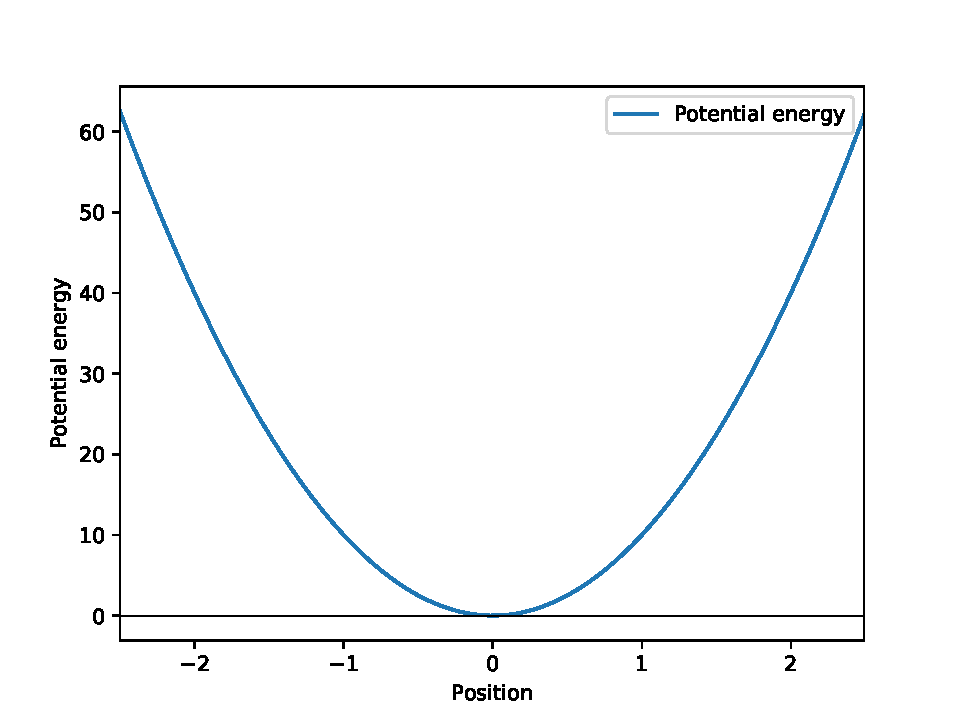
\includegraphics[width=\textwidth]{../imgs/potential/harm_0_0.pdf}
				\caption{Harmonic potential.\newline}
				\label{fig:potential_harm0}
			\end{subfigure}
			\begin{subfigure}[c]{0.32\textwidth}
				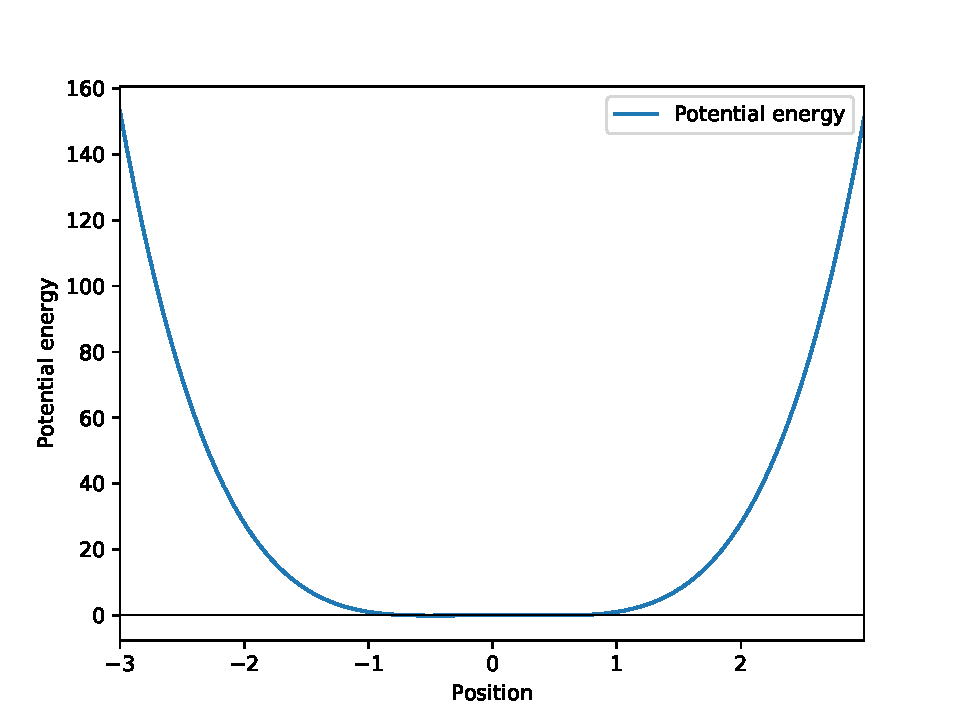
\includegraphics[width=\textwidth]{../imgs/potential/anharm_1_0.pdf}
				\caption{Anharmonic potential, \newline$d=1$.}
				\label{fig:potential_anharm1}
			\end{subfigure}

			\begin{subfigure}[c]{0.32\textwidth}
				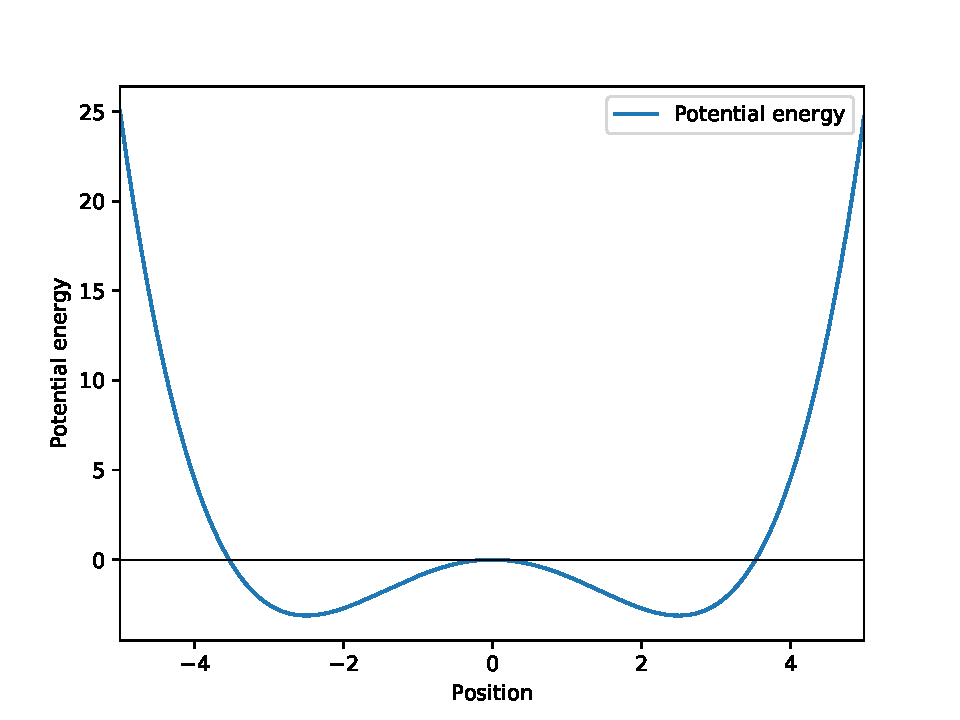
\includegraphics[width=\textwidth]{../imgs/potential/anharm_5_0.pdf}
				\caption{Anharmonic potential, \newline$d=5$.}
				\label{fig:potential_anharm5}
			\end{subfigure}
			\begin{subfigure}[c]{0.32\textwidth}
				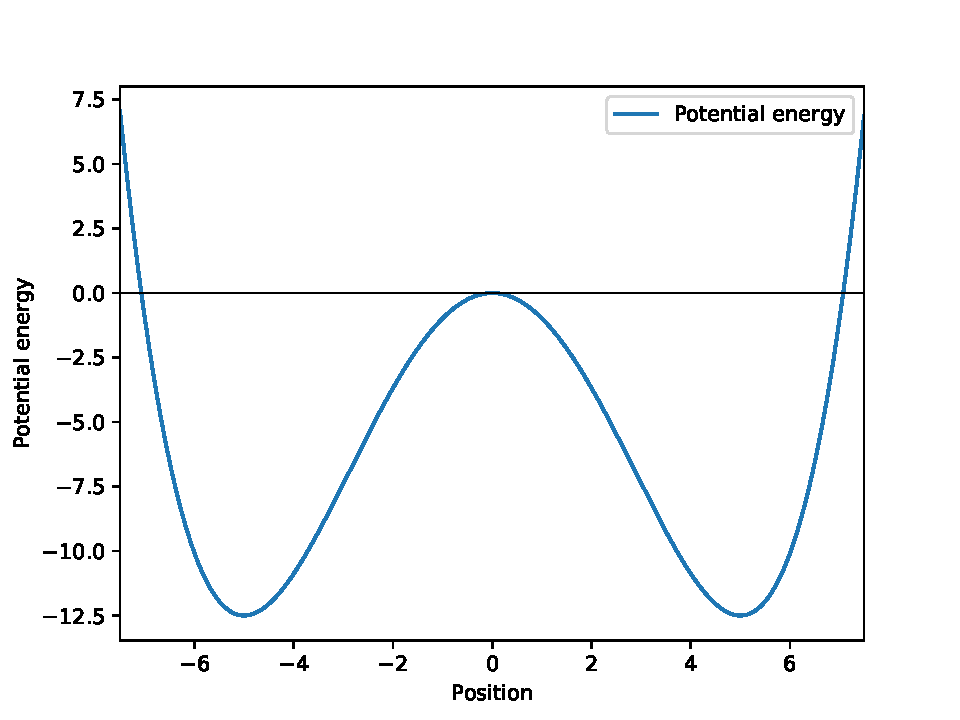
\includegraphics[width=\textwidth]{../imgs/potential/anharm_10_0.pdf}
				\caption{Anharmonic potential, \newline$d=10$.}
				\label{fig:potential_anharm10}
			\end{subfigure}
			\caption{Example potentials.}
			\label{fig:potentials}
		\end{figure}

	\subsection{Verification}
		\label{sec:verification}
		To verify the validity of the code consistency checks were performed.

	\subsubsection{Classical limit}
		One of these consistency checks is the classical limit.
		\begin{figure}[H]
			\centering
			\begin{subfigure}[c]{0.49\textwidth}
				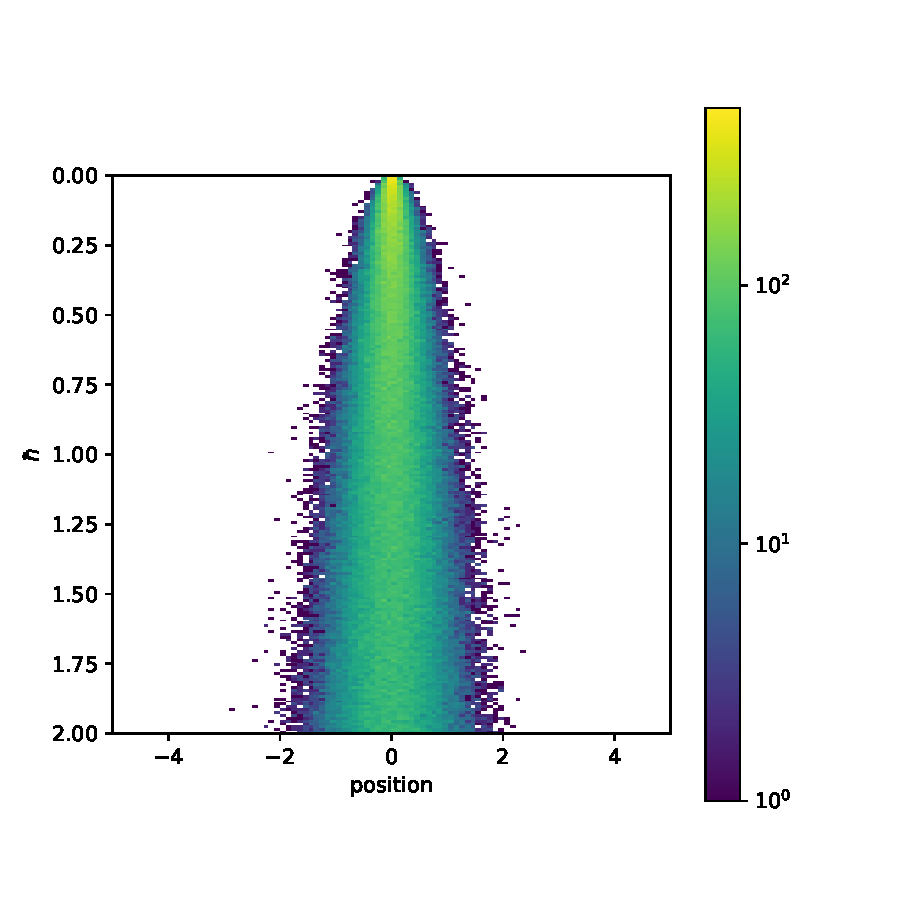
\includegraphics[width=\textwidth]{../imgs/harmonic_oscillator_classical_limit/harmonic_oscillator_10_classical_limit.pdf}
				\caption{Harmonic oscillator.}
				\label{fig:harmonic_oscillator_classical_limit}
			\end{subfigure}
			\begin{subfigure}[c]{0.49\textwidth}
				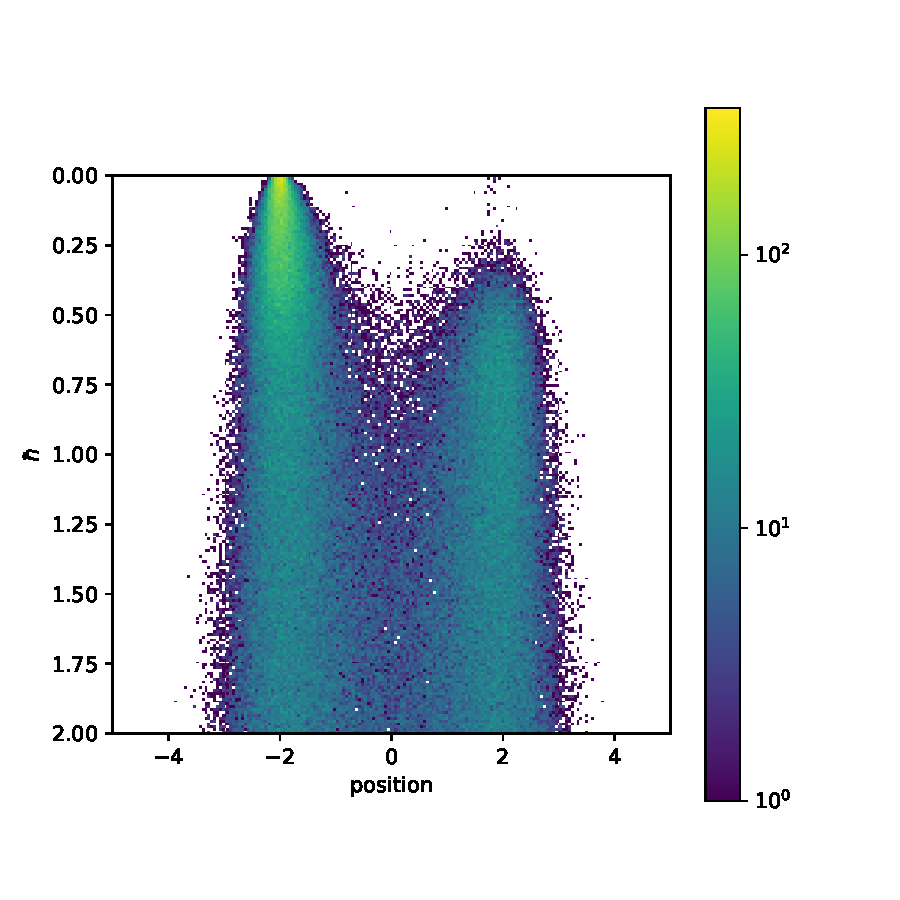
\includegraphics[width=\textwidth]{../imgs/anharmonic_oscillator_classical_limit/anharmonic_oscillator_classical_limit.pdf}
				\caption{Anharmonic oscillator with minima at $\pm2$.}
				\label{fig:anharmonic_oscillator_classical_limit}
			\end{subfigure}
			\caption{Classical limit, probability density for different values of $\hbar$.}
			\label{fig:classical_limits}
		\end{figure}
		In figure \ref{fig:harmonic_oscillator_classical_limit} the standard parameters have been used, on a harmonic potential  with $\mu = 10$ and $\lambda = 0$.
		Similar plots for different values of $m$ are shown in the appendix \ref{sec:harmonic_oscillator_classical_limit_continued}.
		The parameter $\hbar$ has been varied in the range 0 to 2.

		The same data have been generated for the anharmonic oscillator.
		In figure \ref{fig:anharmonic_oscillator_classical_limit} the following parameters have been used: $i = 200$, $N = 1000$, $m = 0.01$, $\mu = -10.0$, $\lambda = -0.125$, corresponding to a position of the minima at $\pm 2.0$.
		The parameter range for the Planck constant is the same as for the harmonic oscillator.
		The initial state has been prepared into the left minimum.

	\subsubsection{Probability density}
		Another test I have performed, is to check the shape of the probability density of the harmonic oscillator.
		\begin{figure}[H]
			\centering
				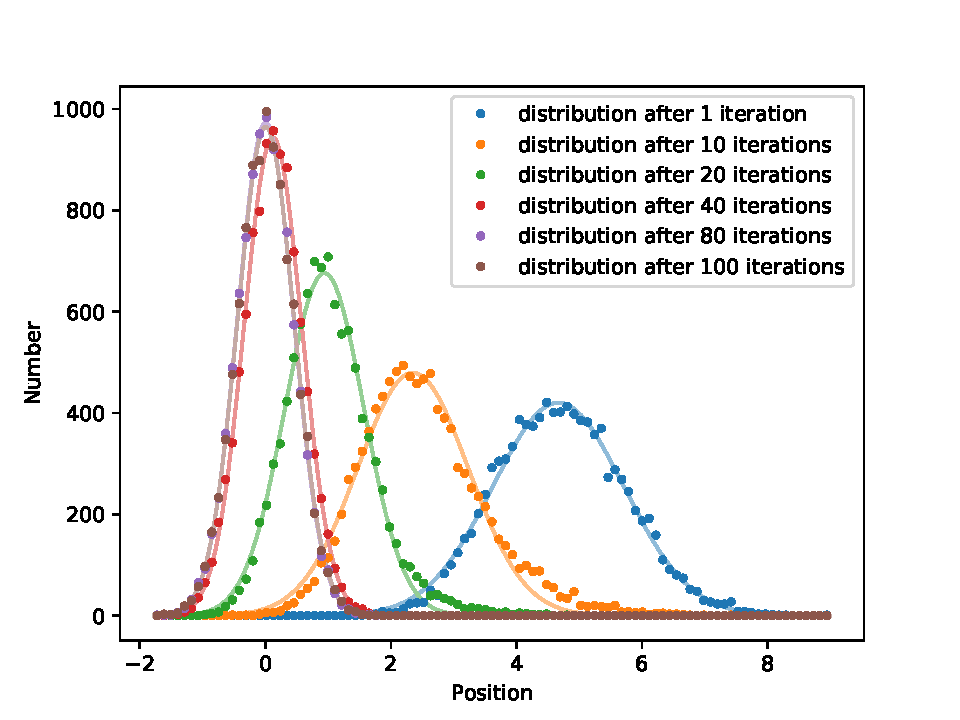
\includegraphics[width=0.5\textwidth]{../imgs/harmonic_oscillator_track/track_10010000_gauss_1_fit.pdf}
			\caption{Probability density for different Metropolis iterations of the harmonic oscillator.}
			\label{fig:harmonic_oscillator_track_10010000_gauss_1_fit}
		\end{figure}
		The parameters used for the plot in figure \ref{fig:harmonic_oscillator_track_10010000_gauss_1_fit} were $i=100$, $N=10000$, $\mu = 10.0$.
		The fits are gaussian distribution functions.
		\\
		To investigate further the probability distribution, quantile-quantile plots can be created to compare the distribution with a gaussian shape.
		\begin{figure}[H]
			\centering
			\begin{subfigure}[c]{0.32\textwidth}
				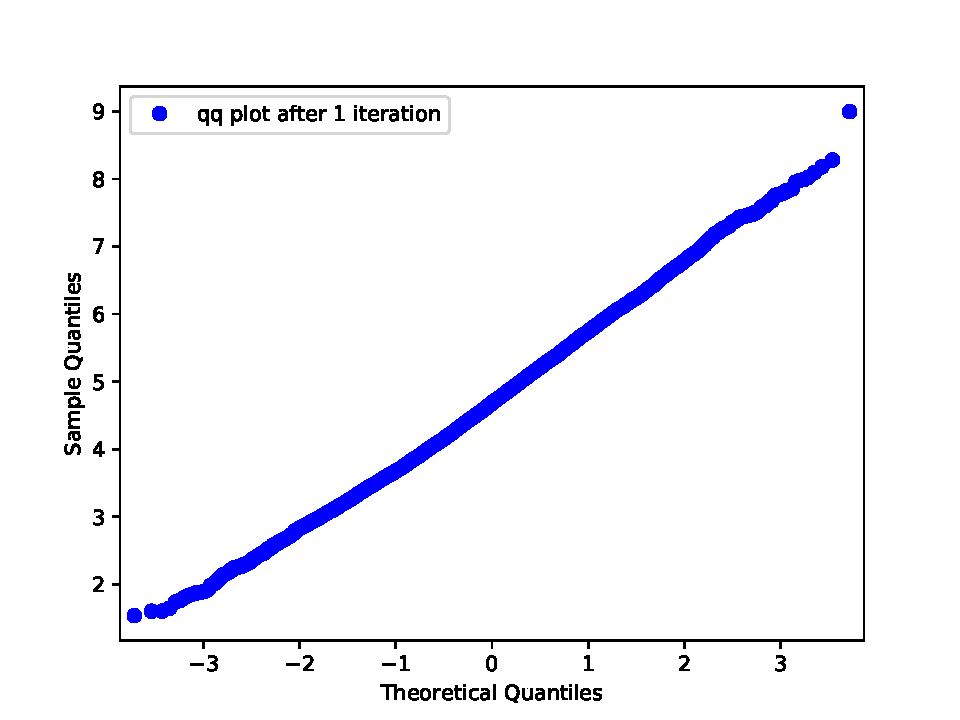
\includegraphics[width=\textwidth]{../imgs/harmonic_oscillator_track/track_10010000_qq_1.pdf}
			\end{subfigure}
			\begin{subfigure}[c]{0.32\textwidth}
				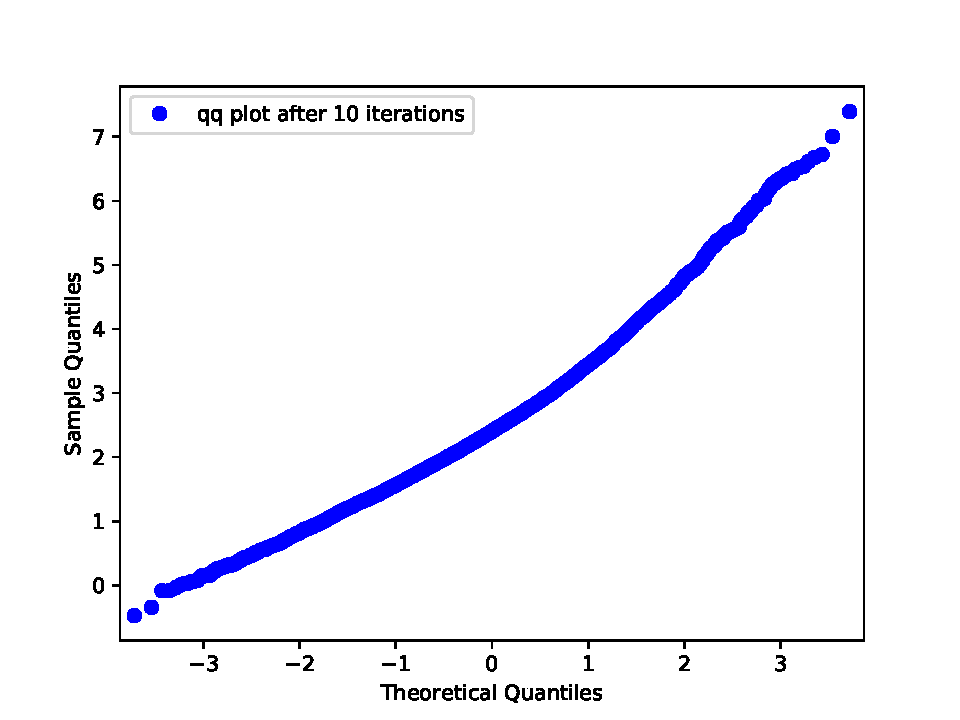
\includegraphics[width=\textwidth]{../imgs/harmonic_oscillator_track/track_10010000_qq_10.pdf}
			\end{subfigure}
			\begin{subfigure}[c]{0.32\textwidth}
				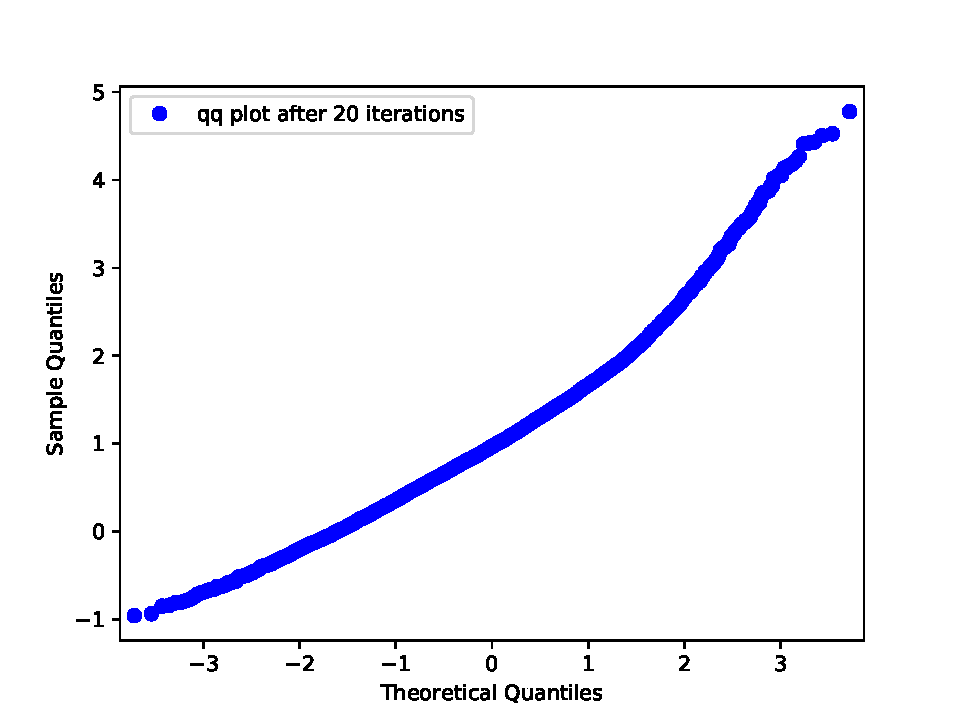
\includegraphics[width=\textwidth]{../imgs/harmonic_oscillator_track/track_10010000_qq_20.pdf}
			\end{subfigure}
			\begin{subfigure}[c]{0.32\textwidth}
				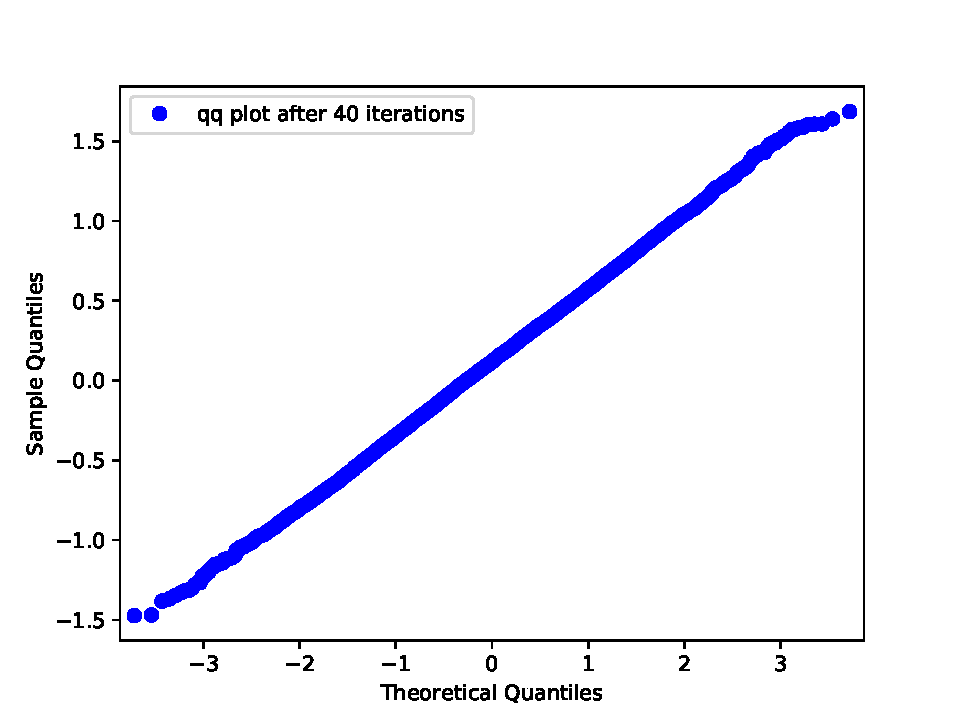
\includegraphics[width=\textwidth]{../imgs/harmonic_oscillator_track/track_10010000_qq_40.pdf}
			\end{subfigure}
			\begin{subfigure}[c]{0.32\textwidth}
				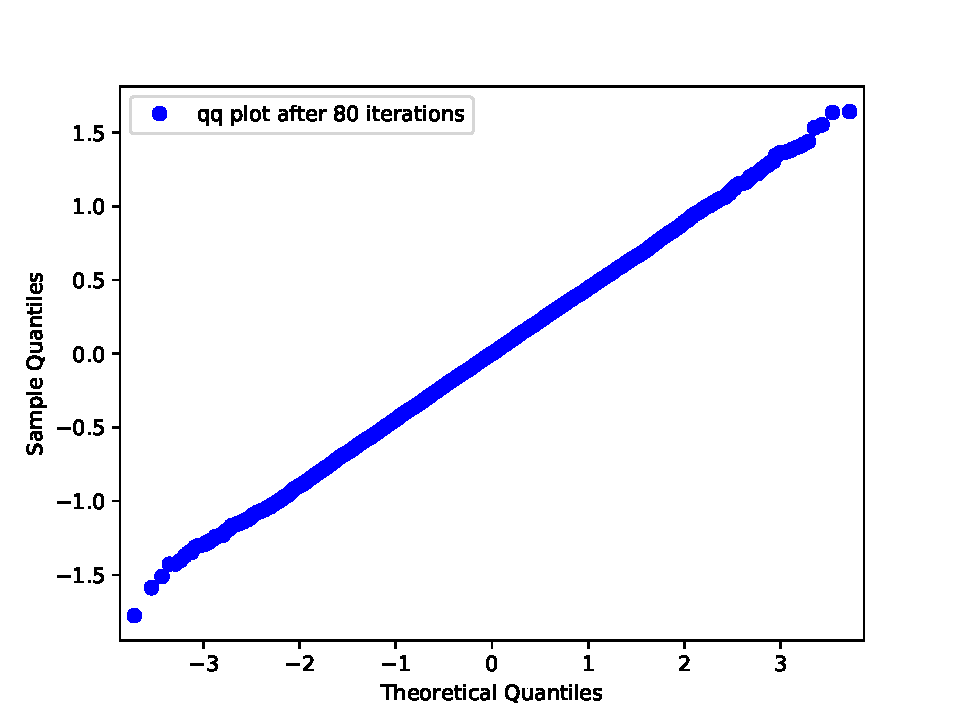
\includegraphics[width=\textwidth]{../imgs/harmonic_oscillator_track/track_10010000_qq_80.pdf}
			\end{subfigure}
			\begin{subfigure}[c]{0.32\textwidth}
				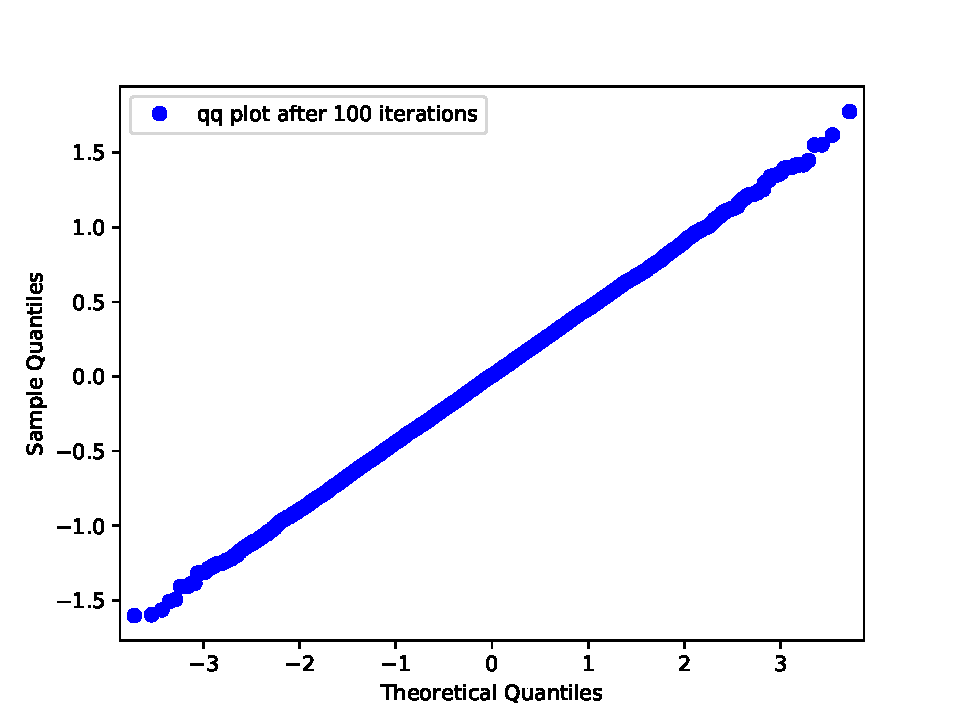
\includegraphics[width=\textwidth]{../imgs/harmonic_oscillator_track/track_10010000_qq_100.pdf}
			\end{subfigure}
			\caption{Thermalisation of the harmonic oscillator from an exited state to the equilibrium.}
			\label{fig:harmonic_oscillator_track_track_10010000_qqs}
		\end{figure}
		In figure \ref{fig:harmonic_oscillator_track_track_10010000_qqs} quantile-quantile plots are shown for the same data and iterations as in figure \ref{fig:harmonic_oscillator_track_10010000_gauss_1_fit}.
		The experimental distribution function was compared to a gaussian distribution function.

	\subsection{Tracks}
		To visualise the behaviour of the particle I have created plots showing the track of the particle.
		\begin{figure}[H]
			\centering
				\begin{subfigure}[c]{0.49\textwidth}
					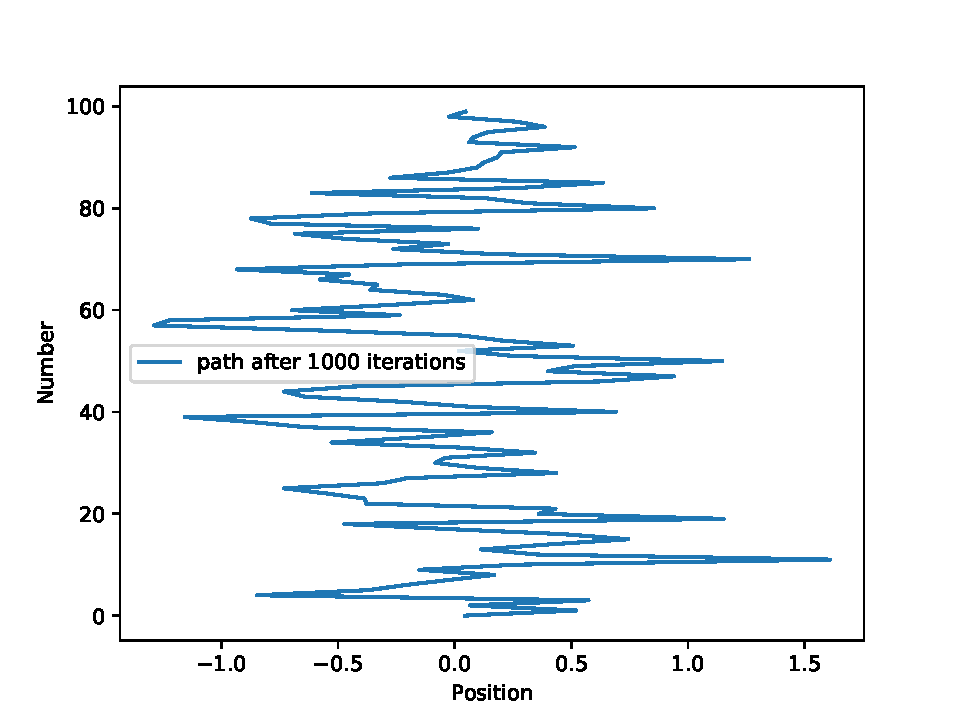
\includegraphics[width=\textwidth]{../imgs/harmonic_oscillator_track/track_1000100_track_1000.pdf}
					\caption{Using a \enquote{light} particle, $m=0.25$}
					\label{fig:harmonic_oscillator_track_1000100_track_1000_light}
				\end{subfigure}
				\begin{subfigure}[c]{0.49\textwidth}
					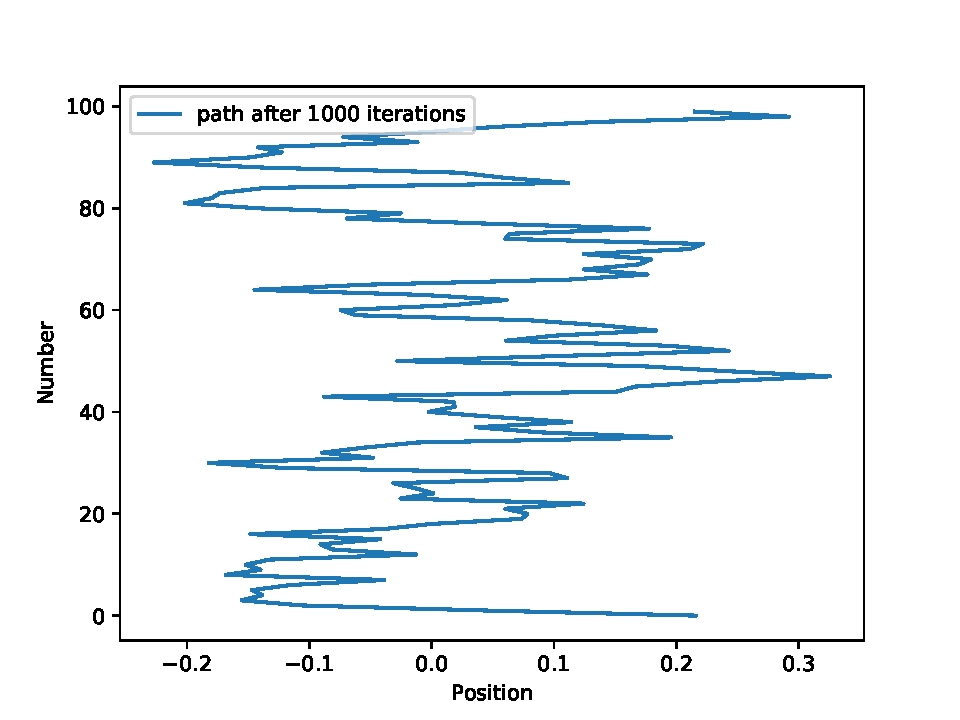
\includegraphics[width=\textwidth]{../imgs/harmonic_oscillator_track/track_1000100_heavy_track_1000.pdf}
					\caption{Using a \enquote{heavy} particle, $m=10.0$}
					\label{fig:harmonic_oscillator_track_1000100_track_1000_heavy}
				\end{subfigure}
			\caption{Typical tracks of the harmonic oscillator. Note the different x scale.}
			\label{fig:harmonic_oscillator_track_1000100_track_1000}
		\end{figure}
		The results for the harmonic oscillator are similar to the tracks shown in figure \ref{fig:harmonic_oscillator_track_1000100_track_1000}.
		The parameters used for the plot were $N=100$, $\mu = 10.0$.
		\begin{figure}[H]
			\centering
				\begin{subfigure}[c]{0.49\textwidth}
					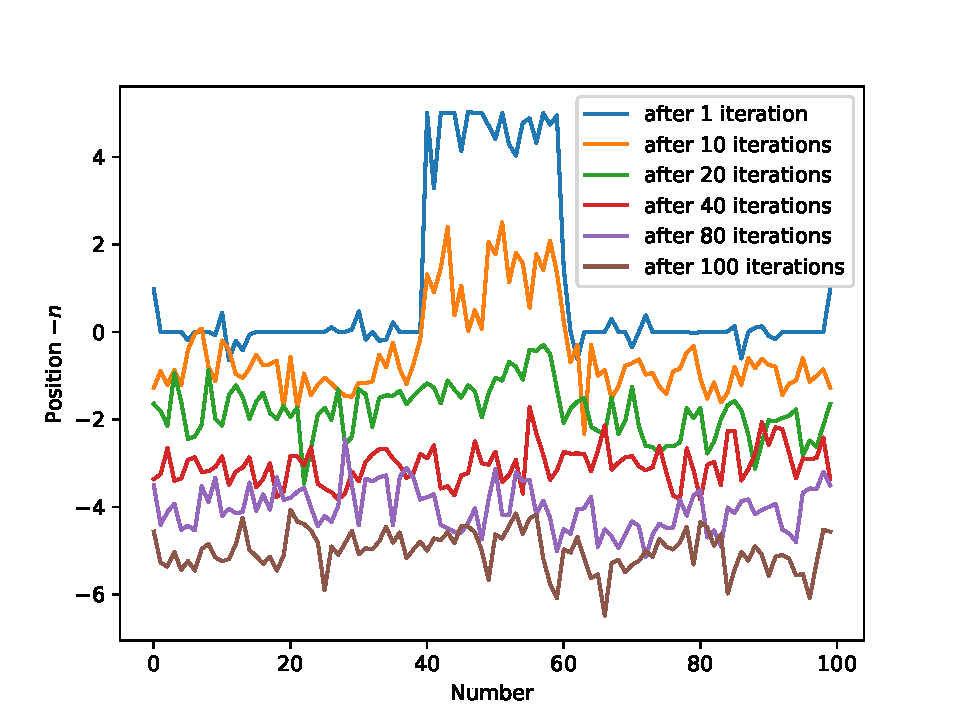
\includegraphics[width=\textwidth]{../imgs/harmonic_oscillator_track/track_100100_step_track_shifted_double.pdf}
					\caption{Typical track of the harmonic oscillator, when initialised with a step function.}
					\label{fig:harmonic_oscillator_track_100100_100100_step_track_shifted_double}
				\end{subfigure}
				\begin{subfigure}[c]{0.49\textwidth}
					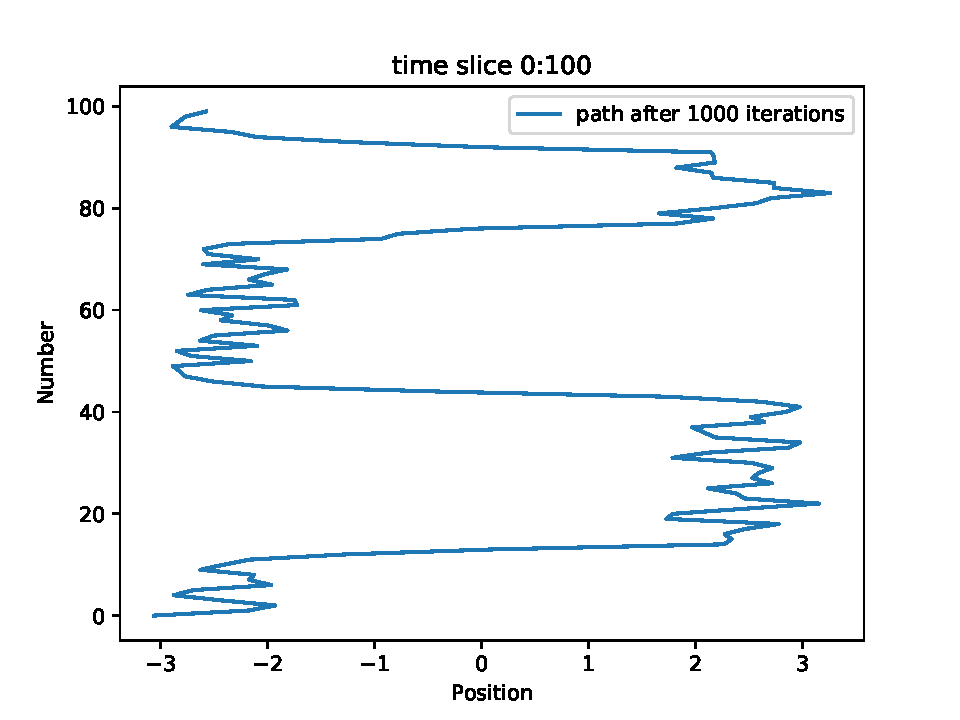
\includegraphics[width=\textwidth]{../imgs/anharmonic_oscillator_track/track_100010005_track_pretty_1000.pdf}
					\caption{Typical track of the anharmonic oscillator, cut to an interesting section.}
					\label{fig:anharmonic_oscillator_track_100010005_track_pretty_1000}
				\end{subfigure}
		\end{figure}
		If the initial state is a step function, a plot similar to \ref{fig:harmonic_oscillator_track_100100_100100_step_track_shifted_double} is obtained.
		The parameters used for the plot were $i=100$, $N=100$, $\mu = 10.0$.
		The individual tracks are shifted by 1 unit in the y direction, the first iteration is not shifted.
		The track has been prepared with a step function with a width of 20\% in the centre and a height of 5.
		The harmonic potential is centred around 0.
		For the anharmonic oscillator similar tracks to the one shown in figure \ref{fig:anharmonic_oscillator_track_100010005_track_pretty_1000} are generated.
		The parameters used for the plot were $i=1000$, $N=1000$ but cut to $N=100$, on an anharmonic potential with $\mu = -10.0$, $\lambda = -0.08$, corresponding to a position of the minima at $\pm 2.5$.

	\subsection{Measurements performed on the simulated data}
	\label{sec:measurements}
	\subsubsection{Classical limit energy}
		\begin{figure}[H]
			\centering
				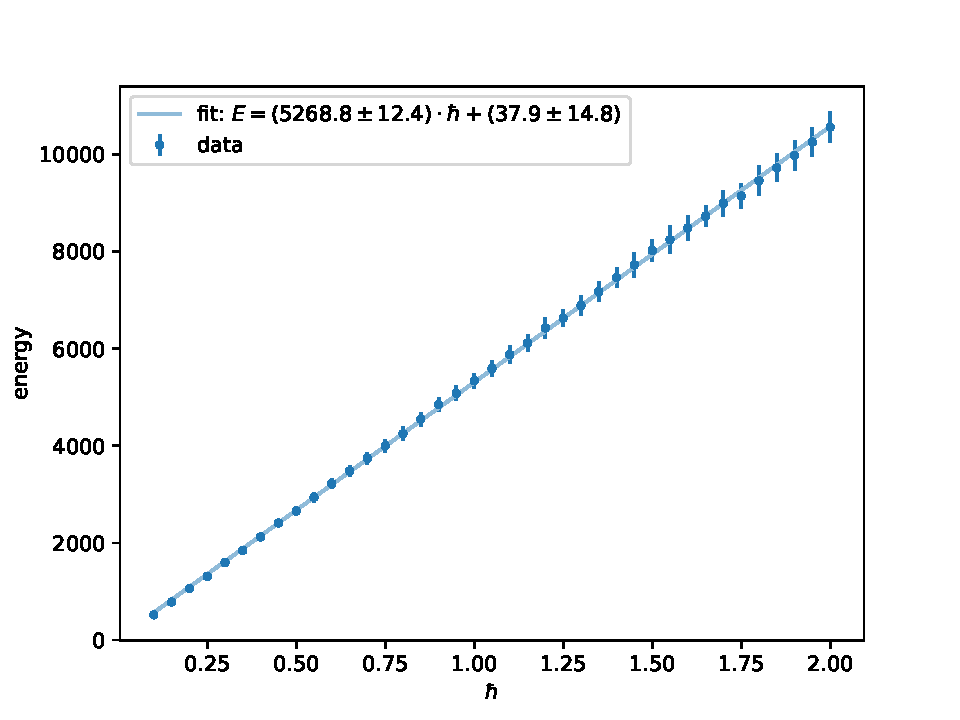
\includegraphics[width=0.5\textwidth]{../imgs/harmonic_oscillator_classical_limit_energy/harmonic_oscillator_10_classical_limit_energy.pdf}
			\caption{Classical limit energy of the harmonic oscillator.}
			\label{fig:harmonic_oscillator_classical_limit_energy}
		\end{figure}
		For plot in figure \ref{fig:harmonic_oscillator_classical_limit_energy} the energy of the harmonic oscillator has been measured depending on the value of $\hbar$.
		The position of the thermalisation has been determined by finding the first sign change of the running mean of the slope of the energy.
		Starting from this position the integrated autocorrelation time has been calculated.
		Then, the data has been blocked into blocks of at least $2 \cdot \tau_{int}$, using the upper bound of the error interval, rounded to the next higher integer, from which the energy and standard deviation of the energy has been measured.
		\\\\
		An example is shown for $\hbar = 1$ in figure \ref{fig:harmonic_oscillator_energy_measurement}.

		\begin{figure}[H]
			\centering
				\begin{subfigure}[c]{0.49\textwidth}
					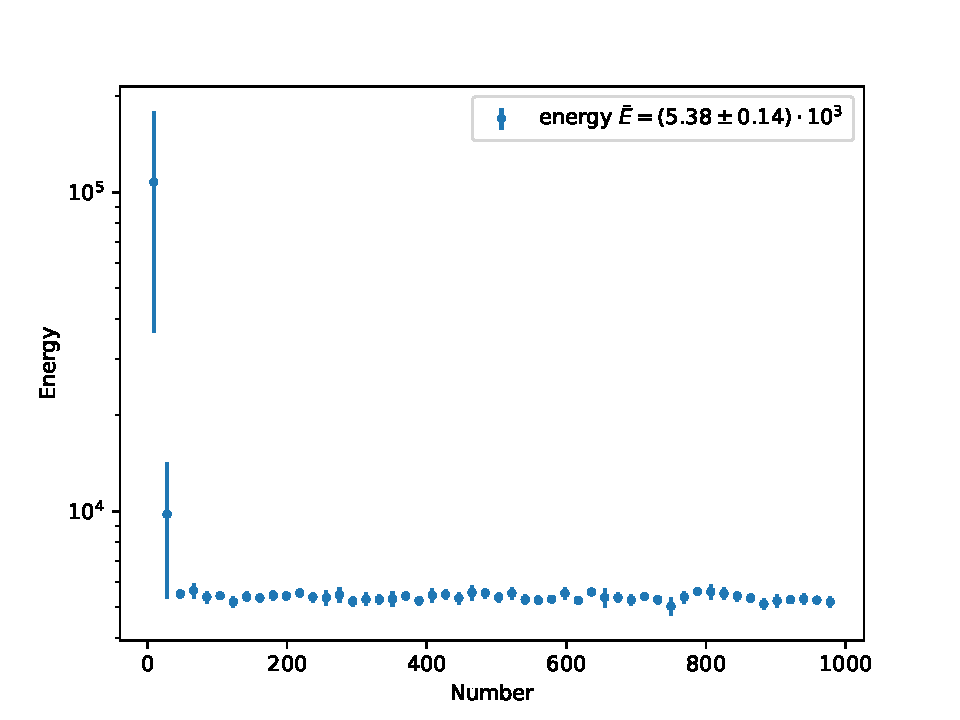
\includegraphics[width=\textwidth]{../imgs/harmonic_oscillator_track/track_10001000_thermalisation_log.pdf}
					\subcaption{Blocked energy measurements}
				\end{subfigure}
				\begin{subfigure}[c]{0.49\textwidth}
					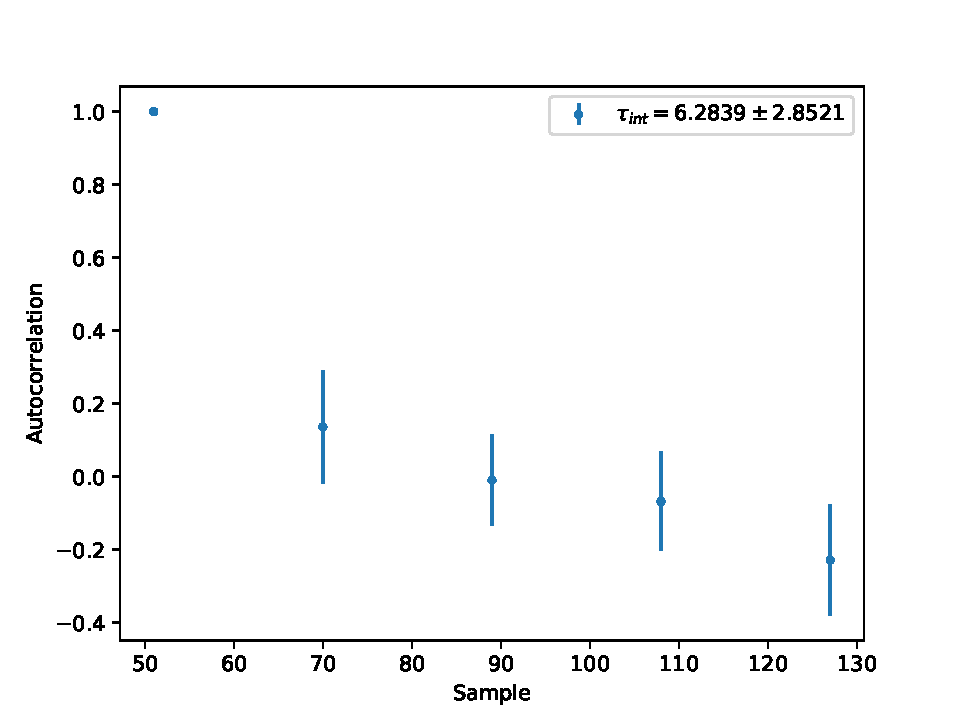
\includegraphics[width=\textwidth]{../imgs/harmonic_oscillator_track/track_10001000_thermalisation_log_autocorrelation.pdf}
					\subcaption{Autocorrelation of the enery measurements}
				\end{subfigure}
			\caption{Measurement of the energy: thermalisation and autocorrelation.}
			\label{fig:harmonic_oscillator_energy_measurement}
		\end{figure}


	\subsubsection{Tunnelling current}
		One of the most interesting features of quantum mechanics is the tunnelling effect.
		\begin{figure}[H]
			\centering
			\begin{subfigure}[c]{0.49\textwidth}
				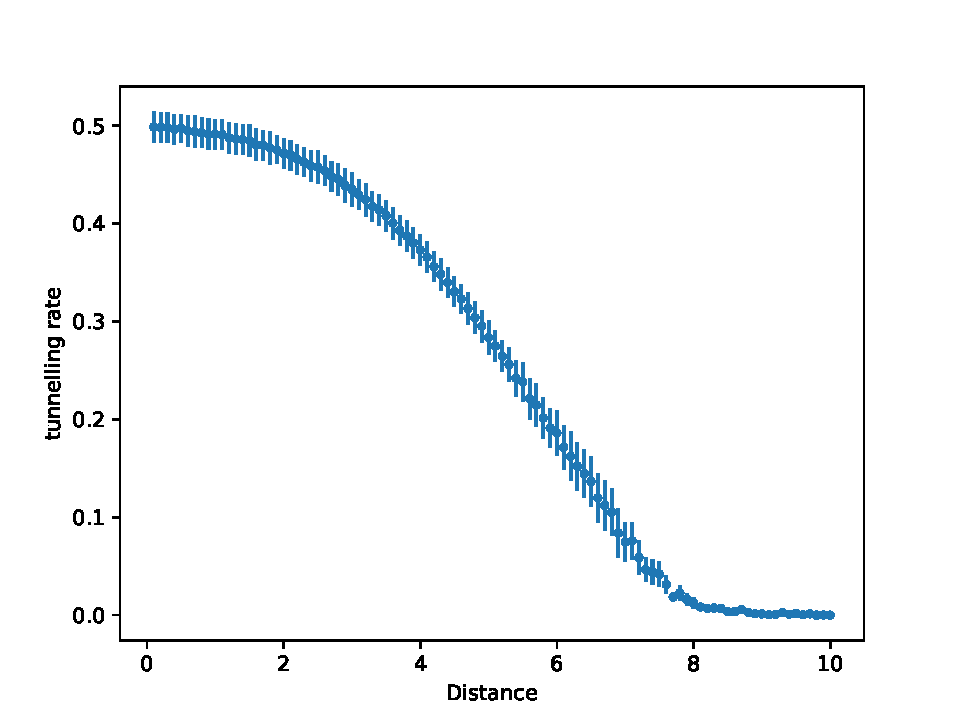
\includegraphics[width=\textwidth]{../imgs/anharmonic_oscillator_lambda_parameter/track_100001000_tunnelling_current.pdf}
				\subcaption{Plotted linearly.}
				\label{fig:anharmonic_oscillator_tunnelling_current_a}
			\end{subfigure}
			\begin{subfigure}[c]{0.49\textwidth}
				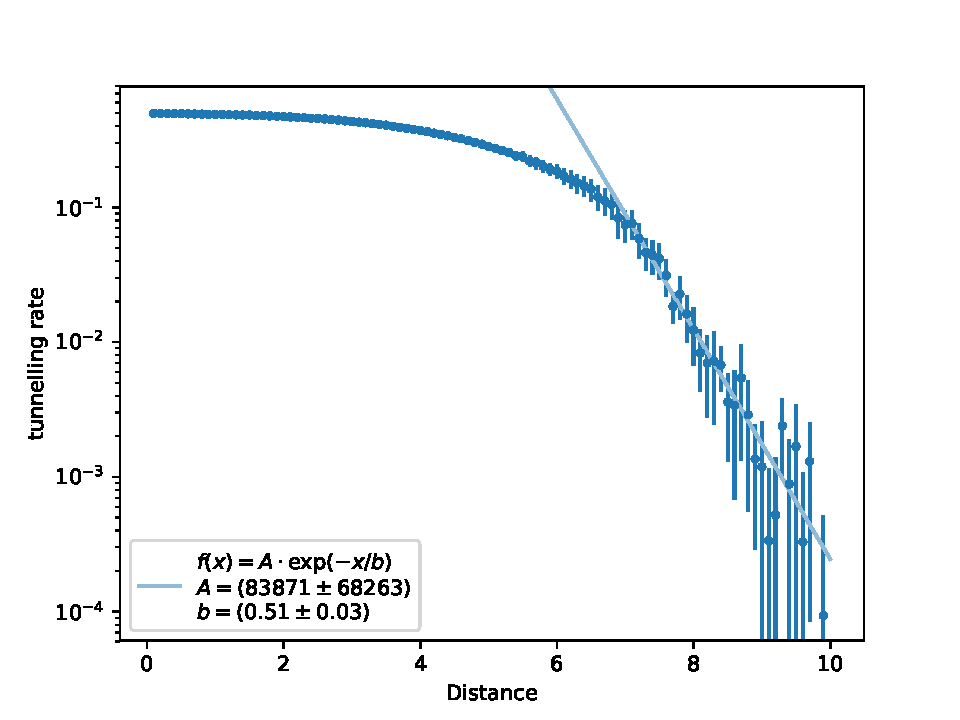
\includegraphics[width=\textwidth]{../imgs/anharmonic_oscillator_lambda_parameter/track_100001000_tunnelling_current_log_fit.pdf}
				\subcaption{Plotted logarithmically with fit.}
				\label{fig:anharmonic_oscillator_tunnelling_current_b}
			\end{subfigure}
			\caption{Tunnelling rate depending on the distance of the classical minima.}
			\label{fig:anharmonic_oscillator_tunnelling_current}
		\end{figure}

		\begin{figure}[H]
			\centering
			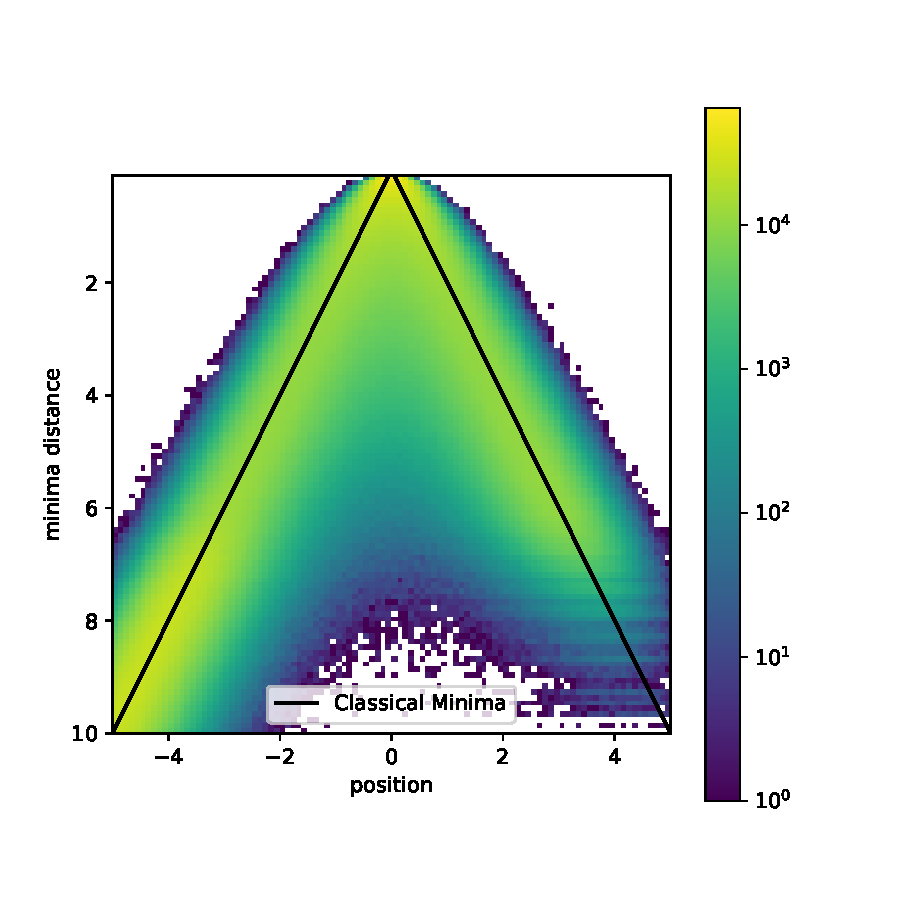
\includegraphics[width=0.5\textwidth]{../imgs/anharmonic_oscillator_lambda_parameter/track_100001000_lambda_parameter.pdf}
			\caption{Probability density depending on the distance of the classical minima.}
			\label{fig:anharmonic_oscillator_lambda_parameter}
		\end{figure}
		For plots in figure \ref{fig:anharmonic_oscillator_tunnelling_current} the following parameters have been used: $i=10000$, $\mu = -10$, $\Delta x_{bin} = 0.1$, $\Delta d = 0.1$, with $\Delta x_{bin}$ and $\Delta d = 0.1$ being the size of the bins in position and distance direction respectively.
		To keep the tunnelling current high enough to be measurable, the mass of the particle for all measurements involving an anharmonic potential has been decreased to $m=0.01$.
		In this case every \nth{15} Metropolis iteration has been used, this has been fixed for every value for $\hbar$.
		Otherwise the number of used values per value of $\hbar$ would not be constant.
		In figure \ref{fig:anharmonic_oscillator_tunnelling_current_b} the same data are plotted half-logarithmically and an exponentially decaying function has been fitted to the data for distances larger than 7.
		The fitted function matches the data quite well, the characteristic length of the exponential function is $b=\SI{0.51 +- 0.03}{}$\unskip.
		Plots \ref{fig:anharmonic_oscillator_tunnelling_current} and \ref{fig:anharmonic_oscillator_lambda_parameter} were produced using the same dataset.
		The initial state has been prepared in the left minimum.

	\subsubsection{Virial theorem}
		It can be shown, that the expectation value of the mean kinetic energy should be equal to the mean potential energy, for the harmonic oscillator, shown in equation \ref{eq:virial}.
		In order to verify this theorem, different simulations have been carried out, varying the mass parameter $m$.
		\begin{figure}[H]
			\centering
				\begin{subfigure}[c]{0.32\textwidth}
					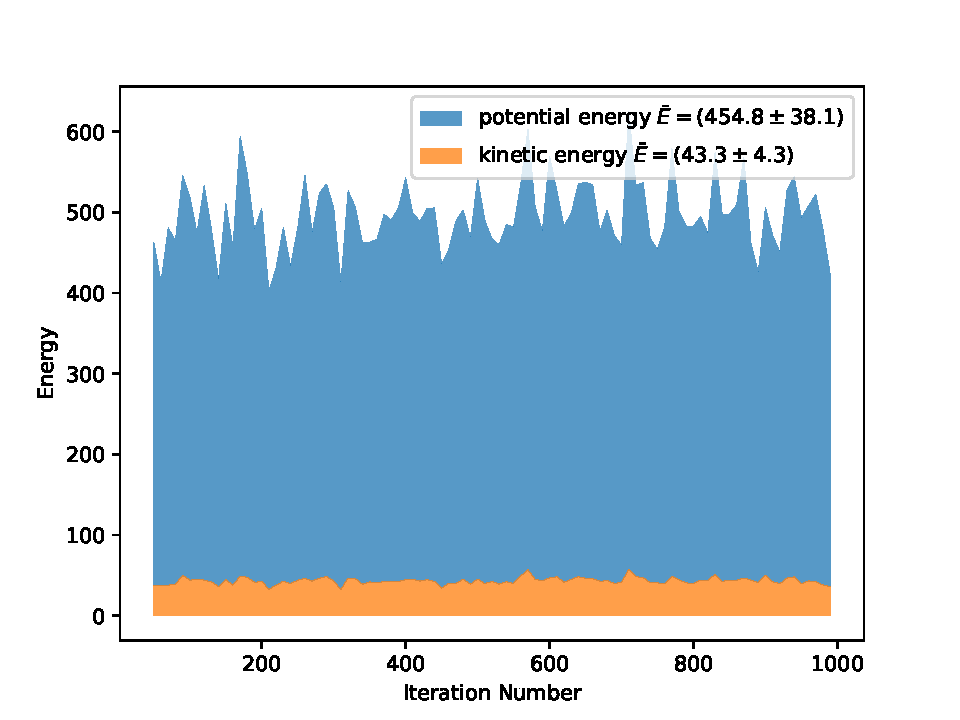
\includegraphics[width=\textwidth]{../imgs/harmonic_oscillator_track/track_1000100_light_virial.pdf}
					\subcaption{Using $m = 0.01$.}
					\label{fig:track_1000100_light_virial}
				\end{subfigure}
				\begin{subfigure}[c]{0.32\textwidth}
					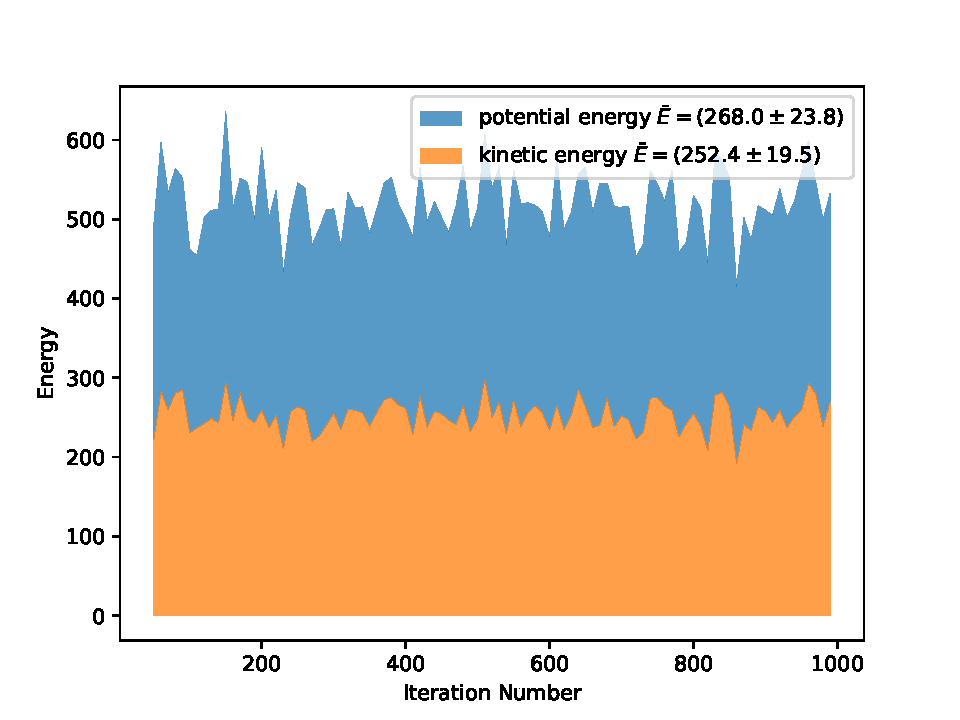
\includegraphics[width=\textwidth]{../imgs/harmonic_oscillator_track/track_1000100_working_virial.pdf}
					\subcaption{Using $m = 0.125$.}
					\label{fig:track_1000100_working_virial}
				\end{subfigure}
				\begin{subfigure}[c]{0.32\textwidth}
					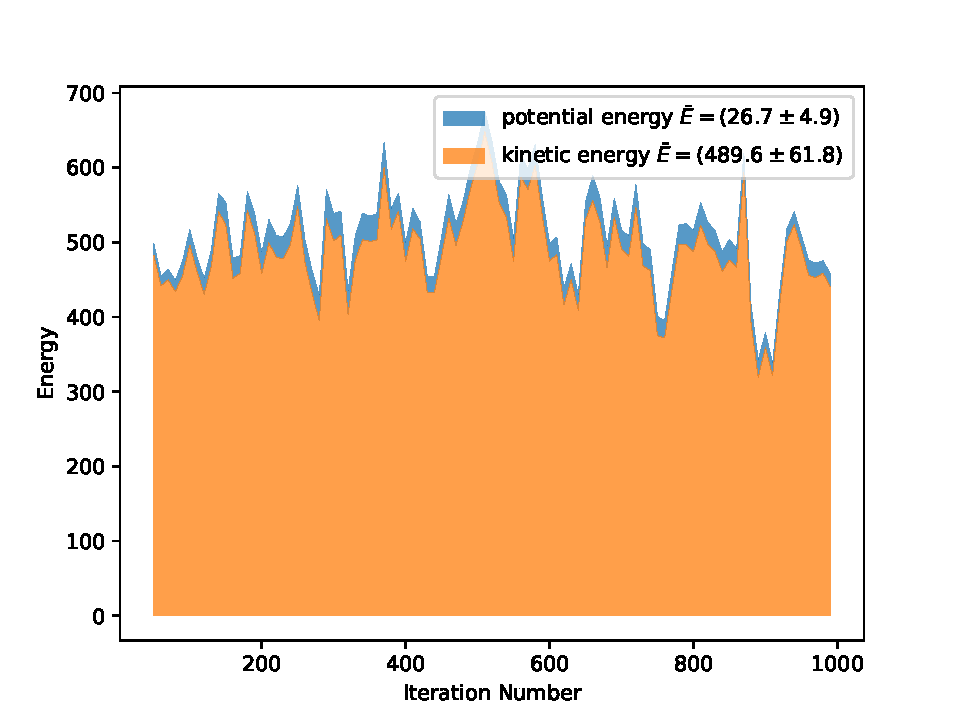
\includegraphics[width=\textwidth]{../imgs/harmonic_oscillator_track/track_1000100_heavy_virial.pdf}
					\subcaption{Using $m = 10.0$.}
					\label{fig:track_1000100_heavy_virial}
				\end{subfigure}
			\caption{Distribution of the total energy into potential and kinetic part.}
			\label{fig:track_1000100_virial}
		\end{figure}
		The plots in figure \ref{fig:track_1000100_virial} show the development of the  kinetic and potential energy separately.
		Due to my findings the ratio between the energies was heavily dependent on the parameters mass $m$ and the time step size $\tau$.

	\section{Discussion}
	\subsection{Verification}
	\subsubsection{Classical limit}
		As shown in figure \ref{fig:harmonic_oscillator_classical_limit}, for $\hbar \rightarrow 0$ the probability density collapses into the minimum of the potential, meeting the expectations from the classical ground state.
		As visible in figure \ref{fig:anharmonic_oscillator_classical_limit}, showing the same plot for the anharmonic oscillator, the behaviour is similar to the harmonic oscillator, so that in the classical limit the probability density only has a significant contribution near the minima of the potential.
		Additionally, it can be observed that there is no significant contribution on the right minimum for $\hbar < 0.3$.
		This is the expected behaviour:
		A classical particle in the ground state in potentials used here should stay at one of the minima in this case at the left minimum where it was initially prepared.
		Additionally, it would be expected that the probability for tunnelling tends to zero, which is observable too.

	\subsubsection{Probability density}
		As shown in figure \ref{fig:harmonic_oscillator_track_10010000_gauss_1_fit}, the initial setup was a gaussian shape, centred around the value 5 with a width of 1, visible in the blue curve.
		This corresponds to an exited state, which then thermalises into the ground state.
		The minimum of the potential is centred around 0.
		The distribution then moves towards this minimum, leading to a deviation from the gaussian shape for iterations 10 and 20.
		After 40 iterations the distribution has nearly reached the centre of the potential and the distribution becomes again gaussian shaped.
		The difference between iterations 80 and 100 is negligible, this indicates that the thermalisation of the centre of mass is done after 80 metropolis iterations.
		From theory it is expected that the probability density is gaussian shaped in the ground state, which is clearly observable as shown below.
		\\\\
		As previously mentioned, it can be seen that the initial setup is a gaussian distribution with centre 5 and width 1.
		In the qq-plots in figure \ref{fig:harmonic_oscillator_track_track_10010000_qqs} for iterations 10 and 20 the deviation from a straight line is clearly visible.
		After the \nth{40} iteration, the centre of the distribution has reached 0 and the qq plot matches a straight line, corresponding to a gaussian distribution.
		\\\\
		The simulated results verify the correctness of the implementation.

	\subsection{Tracks}
		In figure \ref{fig:harmonic_oscillator_track_1000100_track_1000} two typical tracks are shown for different particles.
		In figure \ref{fig:harmonic_oscillator_track_1000100_track_1000_light} a very light particle is used.
		This particle performs huge jumps within the potential.
		In contrast to this, the particle used in \ref{fig:harmonic_oscillator_track_1000100_track_1000_heavy} shows a much more continuous track.
		In figure \ref{fig:harmonic_oscillator_track_100100_100100_step_track_shifted_double} it can be observed how the step function vanishes with increasing Metropolis iteration number.
		The step function disappeared after around 40 Metropolis iterations.
		In figure \ref{fig:anharmonic_oscillator_track_100010005_track_pretty_1000} part of the anharmonic oscillator track can be seen.
		The instants of time when a tunnelling event occurs can be observed.

	\subsection{Measurements performed on the simulated data}
	\subsubsection{Classical limit energy}
		As visible in figure \ref{fig:harmonic_oscillator_classical_limit_energy}, the energy is linearly depending on the value of $\hbar$.
		The fitted function matches very well the data within error limits.
		This is exactly what is expected from exact calculation as in $E = \hbar \omega \left(\frac 12 + n\right)$, where $n$ is the state number, in this case $n = 0$ for the ground state.
		$\omega$ is the proportionality factor, depending on the exact shape of the potential.
		In the classical limit $\hbar \rightarrow 0$ the correct behaviour $E \rightarrow 0$ can be obtained.
		The slope of the fitted linear function is $\frac\omega2=\SI{5268.8 +- 12.4}{}$\unskip.
		The energy at the classical limit $\hbar = 0$ is not directly measurable due to the division by zero, the extrapolation from the linear fit results in $E_0=\SI{37.9 +- 14.8}{}$\unskip.
		This value deviates significantly from the expected value of $0$.
		But comparing the zero value $E_0$ to the typical energy at the \enquote{real} value for $\hbar = 1$, the deviation from zero is very small.

	\subsubsection{Tunnelling current}
		The plot in figure \ref{fig:anharmonic_oscillator_tunnelling_current} shows the rate of tunnelling events divided by the number of opportunities for tunnelling.
		As visible in figure \ref{fig:anharmonic_oscillator_lambda_parameter} real tunnelling only occurs for distances of the minima greater than around 5.
		For smaller distances, the minima of the potential are not clearly separated and transitions are easily possible.
		The corresponding potentials are shown in figure \ref{fig:potentials}, especially in figure \ref{fig:potential_anharm5}.
		For distances greater than 7 it can be observed, that the tunnelling current decays exponentially with increasing distance.
		\\
		\\
		In figure \ref{fig:anharmonic_oscillator_lambda_parameter} the probability density is shown depending on the distance of the classical minima.
		It is obvious, that the distributions for both minima are centred around the positions of the classical minima.
		For higher distances above around 8, the probabilities of finding the particle in the left and right part are not equal.
		The reason for this behaviour is the rapidly decreasing tunnelling current for larger distances of the classical minima.
		Therefore the particle can \enquote{get stuck} in one of the minima.
		Potential future investigations shall take into account an increased number of iterations, to improve the simulation for large distances.
		Additionally, it is clearly visible, that the particle was prepared initially in the left minimum.

	\subsubsection{Virial theorem}
		According to equation \ref{eq:virial} the ratio between kinetic and potential energy is expected to be equal.
		The ratio between the two parts should therefore be around 1.
		However, this could not be reproduced by the simulation, since the ratios are dependent on the mass.
		\\
		The measured ratios are within error boundaries equal to $10.0$, $1.0$ and $0.05$ respectively.
		This deviation from the expected ratio of 1 has to be therefore assessed as very significant.
		The scope of this project did not allow further examinations on this very item.

	\section{Summary and Outlook}
		The simulation results meet the theoretical expectations to a high extend.
		As presented in section \ref{sec:verification}, the produced data do behave as expected when using the classical limit.
		Furthermore, the probability density follows a gaussian distribution as predicted and the variation of parameters as the mass $m$ have shown the expected behaviour.
		The results of section \ref{sec:measurements} validate, that the energy of the harmonic oscillator is linearly dependent on $\hbar$.
		Additionally, the tunnelling current decays rapidly with increasing distance between the minima, as expected.
		\\
		The harmonic and anharmonic oscillators served well as toy models to investigate interesting quantum mechanical phenomena like the tunnelling effect.
		\\
		Further investigations are recommended to determine the reasons why the Virial theorem is not fulfilled for every set of parameters.
		\\
		The Metropolis-Hastings algorithm is in principle easily applicable to systems of higher dimensions, for example the effort to implement the H$_2^+$-ion in this way would be not that large.
		The software provided with this project could serve as a framework for such applications with only minor changes required.
		\\\\\\\\\\\\

	\section{Acknowledgements}
		I would like to thank Matthias Fischer for the very helpful support and Simon Schlepphorst for helping setting up the makefile.

	\newpage
	\begin{thebibliography}{widestlabel}
		\bibitem{bender} C. M. Bender and T. T. Wu, \textit{Anharmonic oscillator}, Phys. Rev. (2) \textbf{184}, 1231–1260 (1969).
		\bibitem{rushka_freericks} M. Rushka J. K. Freericks, \textit{A Completely Algebraic Solution of the Simple Harmonic Oscillator}, arXiv:1912.08355 [quant-ph] (2019).
		\bibitem{creutz_freedman} M. Creutz and B. Freedman, \textit{A statistical approach to quantum mechanics}, Annals of Physics, \textbf{132}, 427-462 (1981).
		\bibitem{rodgers_raes} R. Rodgers and L. Raes, \textit{Monte Carlo simulations of harmonic and anharmonic oscillators in discrete Euclidean time}, DESY Summer Student Programme (2014).
		\bibitem{wick} G. C. Wick, \textit{Properties of Bethe-Salpeter Wave Functions}, Physical Review. \textbf{96} 1124–1134 (1954).
		\bibitem{carinena_falceto_ranada} J. F. Cari\~{n}ena, F. Falceto and M. F. Ra\~{n}ada, \textit{A geometric approach to a generalized virial theorem}, arXiv:1209.4584 [math-ph] (2012).
		\bibitem{github} Public Github repository: Harmonic Oscillator, Benedikt Otto (s6beotto), \\\url{https://github.com/s6beotto/Harmonic-Oscillator}.
		\bibitem{latexrun} Public Github repository: latexrun, Austin Clements (aclements), \\\url{https://github.com/aclements/latexrun}.
	\end{thebibliography}
	\appendix

	\section{Directory structure}
	\label{sec:directory_structure}
	\subsection{Data generation}
	\begin{figure}[H]
		\centering
		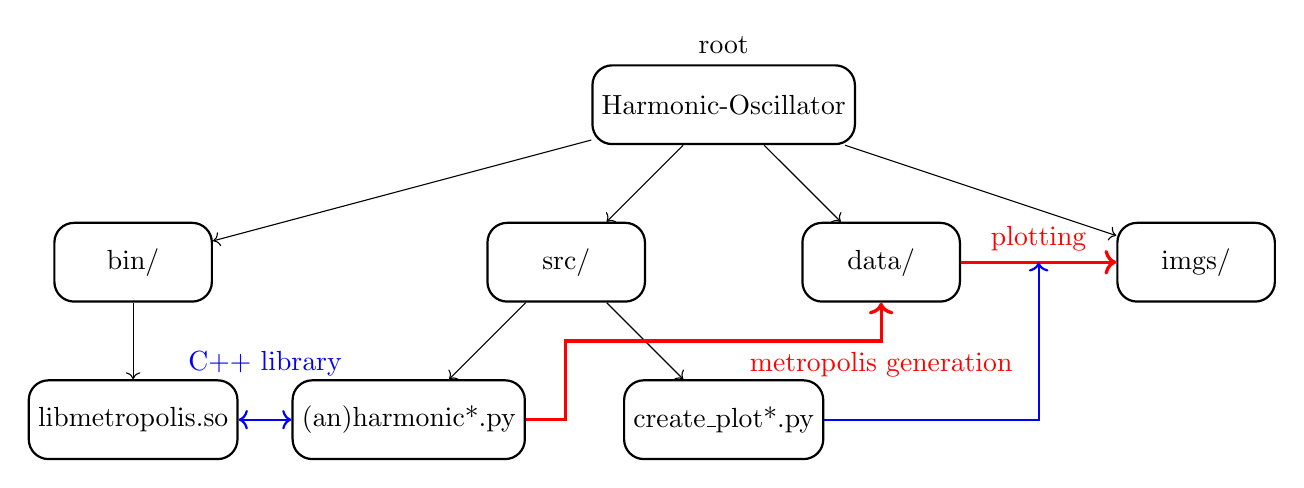
\begin{tikzpicture}
		\draw[color=black, thick]
		node[draw,minimum width=2cm,minimum height=1cm,label=root,rounded corners=0.25cm] (root) at (0, 0){Harmonic-Oscillator}
		node[draw,minimum width=2cm,minimum height=1cm,rounded corners=0.25cm] (bin) at (-7.5, -2){bin/}
		node[draw,minimum width=2cm,minimum height=1cm,rounded corners=0.25cm] (bin_metropolis) at (-7.5, -4){libmetropolis.so}
		node[draw,minimum width=2cm,minimum height=1cm,rounded corners=0.25cm] (src) at (-2, -2){src/}
		node[draw,minimum width=2cm,minimum height=1cm,rounded corners=0.25cm] (src_create) at (-4, -4){(an)harmonic*.py}
		node[draw,minimum width=2cm,minimum height=1cm,rounded corners=0.25cm] (src_plot) at (0, -4){create\_plot*.py}
		node[draw,minimum width=2cm,minimum height=1cm,rounded corners=0.25cm] (data) at (2, -2){data/}
		node[draw,minimum width=2cm,minimum height=1cm,rounded corners=0.25cm] (imgs) at (6, -2){imgs/};
		\draw [->] (root) -- (bin);
			\draw [->] (bin) -- (bin_metropolis);
		\draw [->] (root) -- (src);
			\draw [->] (src) -- (src_create);
			\draw [->] (src) -- (src_plot);
		\draw [->] (root) -- (data);
		\draw [->] (root) -- (imgs);
		\draw [<->, thick, blue] (bin_metropolis) -- (src_create) node[midway,above=12] {C++ library};
		\draw [->, very thick, red] (src_create.east) -| ++(0.5, 1) -| (data) node[midway,below] {metropolis generation};
		\draw [->, very thick, red] (data) -- (imgs) node[midway,above] {plotting};
		\draw [->, thick, blue] (src_plot.east) -| (4, -2);
		\end{tikzpicture}
		\caption{Directory structure of the project for data generation.}
		\label{fig:scheme_dirs_data_generation}
	\end{figure}

	\subsection{Report generation}
	\begin{figure}[H]
		\centering
		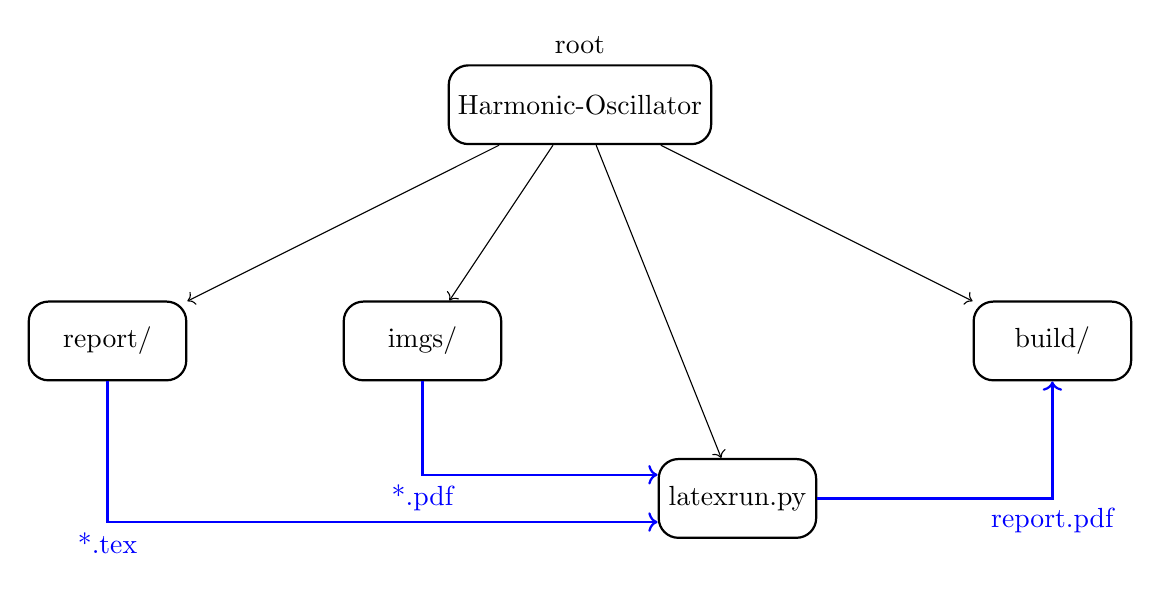
\begin{tikzpicture}
		\draw[color=black, thick]
		node[draw,minimum width=2cm,minimum height=1cm,label=root,rounded corners=0.25cm] (root) at (0, 0){Harmonic-Oscillator}
		node[draw,minimum width=2cm,minimum height=1cm,rounded corners=0.25cm] (report) at   (-6,  -3){report/}
		node[draw,minimum width=2cm,minimum height=1cm,rounded corners=0.25cm] (imgs) at     (-2, -3){imgs/}
		node[draw,minimum width=2cm,minimum height=1cm,rounded corners=0.25cm] (latexrun) at (2,  -5){latexrun.py}
		node[draw,minimum width=2cm,minimum height=1cm,rounded corners=0.25cm] (build) at    (6,  -3){build/};
		\draw [->] (root) -- (report);
		\draw [->] (root) -- (imgs);
		\draw [->] (root) -- (latexrun);
		\draw [->] (root) -- (build);
		\draw [<-, thick, blue] (latexrun.west) + (0,-3mm) -| (report.south) node[midway,below] {*.tex};
		\draw [<-, thick, blue] (latexrun.west) + (0, 3mm) -| (imgs.south)   node[midway,below] {*.pdf};
		\draw [->, thick, blue] (latexrun) -| (build.south)                  node[midway,below] {report.pdf};
		\end{tikzpicture}
		\caption{Directory structure of the project for report generation.}
		\label{fig:scheme_dirs_report_generation}
	\end{figure}
	The file \verb!latexrun.py! is taken from \cite{latexrun}.
	Every process in the generation of this report is controlled by a makefile.
	\section{harmonic oscillator: classical limit}
	\label{sec:harmonic_oscillator_classical_limit_continued}
	\begin{figure}[H]
		\centering
			\begin{subfigure}[c]{0.32\textwidth}
				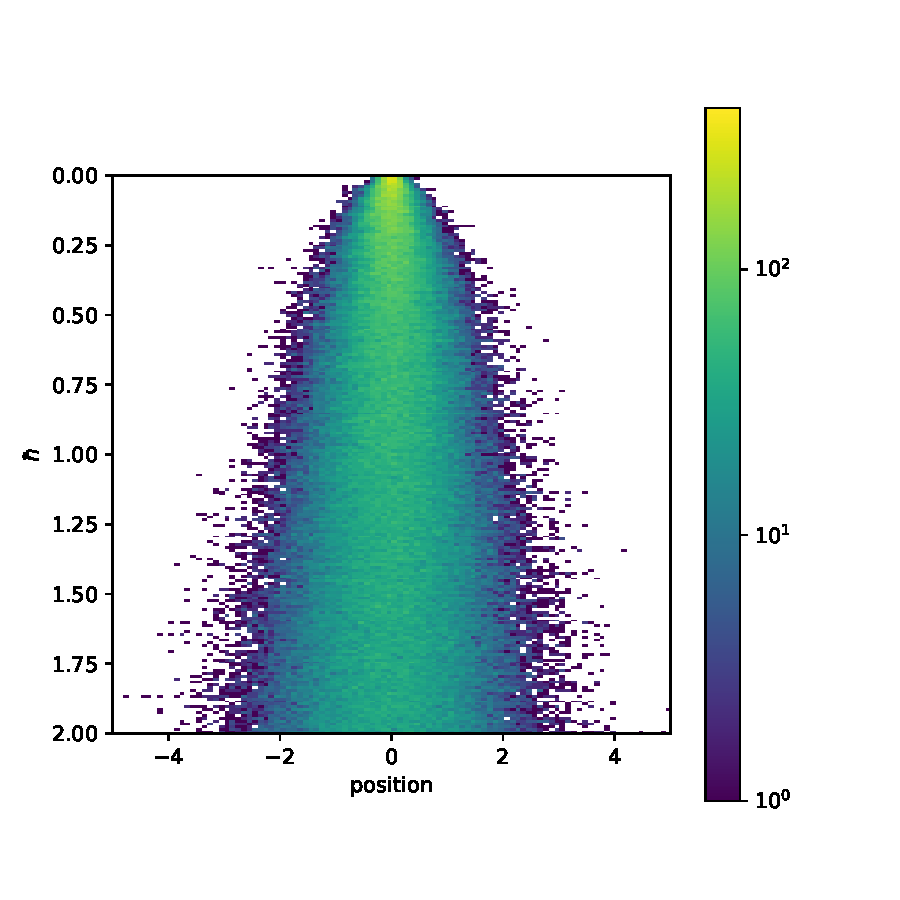
\includegraphics[width=\textwidth]{../imgs/harmonic_oscillator_classical_limit/harmonic_oscillator_1_classical_limit.pdf}
				\subcaption{Using $m = 1$.}
				\label{fig:harmonic_oscillator_1_classical_limit_continued}
			\end{subfigure}
			\begin{subfigure}[c]{0.32\textwidth}
				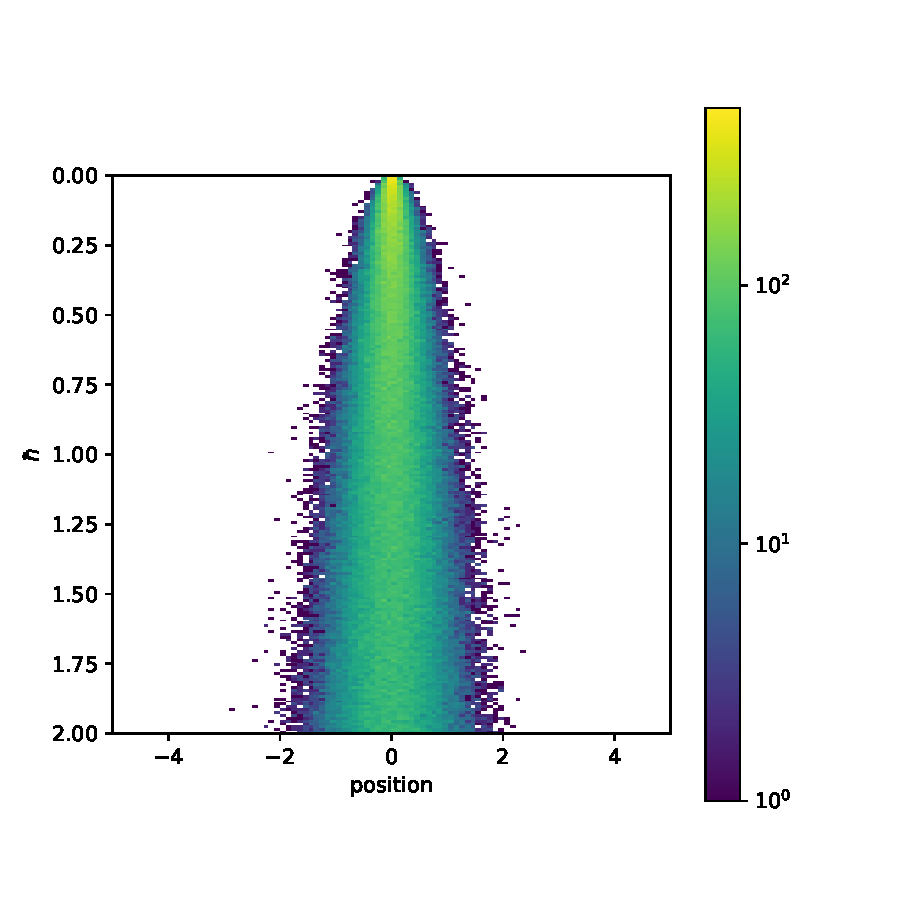
\includegraphics[width=\textwidth]{../imgs/harmonic_oscillator_classical_limit/harmonic_oscillator_10_classical_limit.pdf}
				\subcaption{Using $m = 10$.}
				\label{fig:harmonic_oscillator_10_classical_limit_continued}
			\end{subfigure}
			\begin{subfigure}[c]{0.32\textwidth}
				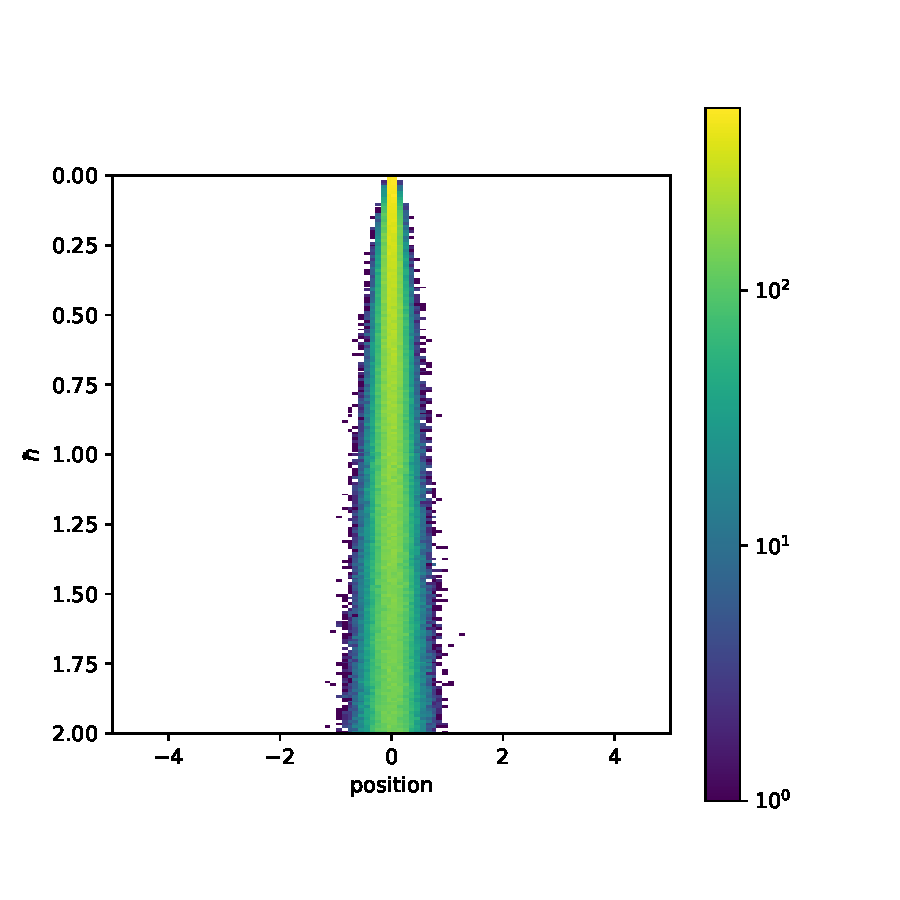
\includegraphics[width=\textwidth]{../imgs/harmonic_oscillator_classical_limit/harmonic_oscillator_100_classical_limit.pdf}
				\subcaption{Using $m = 100$.}
				\label{fig:harmonic_oscillator_100_classical_limit_continued}
			\end{subfigure}
		\caption{Classical limit of the harmonic oscillator, continued.}
		\label{fig:harmonic_oscillator_classical_limit_continued}
	\end{figure}
\end{document}